%
% File acl2020.tex
%
%% Based on the style files for ACL 2020, which were
%% Based on the style files for ACL 2018, NAACL 2018/19, which were
%% Based on the style files for ACL-2015, with some improvements
%%  taken from the NAACL-2016 style
%% Based on the style files for ACL-2014, which were, in turn,
%% based on ACL-2013, ACL-2012, ACL-2011, ACL-2010, ACL-IJCNLP-2009,
%% EACL-2009, IJCNLP-2008...
%% Based on the style files for EACL 2006 by 
%%e.agirre@ehu.es or Sergi.Balari@uab.es
%% and that of ACL 08 by Joakim Nivre and Noah Smith

\documentclass[11pt,a4paper]{article}
\usepackage[hyperref]{acl2020}
\usepackage{times}
\usepackage{latexsym}
\renewcommand{\UrlFont}{\ttfamily\small}

% This is not strictly necessary, and may be commented out,
% but it will improve the layout of the manuscript,
% and will typically save some space.
\usepackage{microtype}

%\aclfinalcopy % Uncomment this line for the final submission
%\def\aclpaperid{***} %  Enter the acl Paper ID here

%=======================Additional  Packages ==============%
\usepackage{adjustbox}
\usepackage{tikz}
\usetikzlibrary{arrows,automata}
\usetikzlibrary{positioning}
\usepackage{mypackages}

\usepackage{latexsym,amssymb,amsfonts,amsmath}
\usepackage{pstricks,verbatim,url,float}
\usepackage{makeidx}
\usepackage{multirow}

\usepackage{parskip}
\usepackage{microtype}
\usepackage{tipa}
\usepackage{algorithm2e}
\usepackage{microtype}
\usepackage{linguex}
\usepackage{stmaryrd}
\usepackage{amsthm}
%\usepackage{amssymb}
%\usepackage{amsmath}
\usepackage{graphicx}
\usepackage{float}
\usepackage{gastex}
\usepackage[normalem]{ulem}

%=======================Additional  Commands ==============%
\usepackage{mycommands}
\newcommand{\unproject}[1]{\ensuremath{\downarrow #1}}
%\newcommand{\comment}[3]{\textbf{From:} {#1} \textbf{To:} {#2} \textcolor{red}{#3}}
\newcommand{\etal}{\emph{et al. }}

%function macros
%A collection of macros for mathy stuff
%
%Last edit Dec 16 2014
%
%Much stolen from jim/CLmacros.tex

%Short \textnormal
\newcommand{\tn}[1]{\textnormal{#1}}

%**Notation

%Enclosures
%tuples
\newcommand{\Tup}[1]{{\left\langle#1\right\rangle}}
\newcommand{\tup}[1]{\langle{#1}\rangle}
%sets
\newcommand{\Set}[1]{\left\{#1\right\}}
%\newcommand{\set}[1]{\{#1\}}
%brackets
\newcommand{\Brac}[1]{\left[#1\right]}
\newcommand{\brac}[1]{[#1]}
%parens
\newcommand{\Paren}[1]{\left(#1\right)}
\newcommand{\paren}[1]{(#1)}
%cardinality
\newcommand{\Card}[1]{\left|#1\right|}
\newcommand{\card}[1]{|#1|}

%Common notational thingies
\def\natn{\mathbb{N}}
\def\treq{\triangleq}

\newcommand\pow[1]{\ensuremath{\mathcal{P}(#1)}}       %powerset
\newcommand\powf[1]{\ensuremath{\mathcal{P}_{fin}(#1)}} %set of all finite sets
\newcommand\powk[2]{\ensuremath{\mathcal{P}_{=#1}(#2)}} %set of sets of cardinality k
\def\Tau{\ensuremath{\tn{T}}}
\def\Alpha{\ensuremath{\tn{A}}}

%Equals and iff for definitions
\def\defeq{\mathrel{\buildrel \mbox{\footnotesize def} \over =}}
\def\defiff{\mathrel{\buildrel \mbox{\footnotesize def} \over \liff}}
\def\defequiv{\mathrel{\buildrel \mbox{\footnotesize def} \over \equiv}}

%Logic
\def\land{\wedge}                         %and
\def\fatimp{\ensuremath{\Rightarrow}}     %implication (for teh meta)
\def\fatbackimp{\ensuremath{\Leftarrow}}  %implication (left) (for teh meta)
\def\fatiff{\ensuremath{\Leftrightarrow}} %iff (for teh meta)
\def\limp{\rightarrow}                    %implication (regular)
\let\liff=\leftrightarrow                 %iff (regular)
\def\sats{\models}                        %satisfies

%Models
\newcommand{\sW}{\ensuremath{\mathcal{W}}}     %Word model
\newcommand{\sU}{\ensuremath{\mathcal{U}}}     %Word model (U)
\newcommand{\sX}{\ensuremath{\mathcal{X}}}     %Word model (X)
\newcommand{\sA}{\ensuremath{\mathcal{A}}}     %Association model

\newcommand{\SW}{\ensuremath{\mathbb{W}}}      %Set of word models
\newcommand{\SU}{\ensuremath{\mathbb{U}}}      %Set of word models (U)
\newcommand{\SX}{\ensuremath{\mathbb{X}}}      %Set of word models (X)
\newcommand{\SA}{\ensuremath{\mathbb{A}}}      %Set of association models

\newcommand{\Mod}[1][]{\ensuremath{\mathbf{Mod}_{#1}}}     %Model [structure]
\newcommand{\Th}{\ensuremath{\mathbf{Th}}}                %Theory

\newcommand{\ladj}[1][]{\mathrel{\triangleleft_{#1}}}     %Adjacency (immediate precedence); [tier]
\newcommand{\lltpred}[1][]{\mathrel{\triangleleft^+_{#1}}}%Less than precedence optional; [tier]
\newcommand{\lpred}[1][]{\mathrel{\triangleleft^*_{#1}}}  %Full precedence optional; [tier]
\newcommand{\assoc}{\vartriangle}                         %Immediate association
\newcommand{\lequals}{\approx}                            %Equivalence for variables

%Automata
\newcommand{\nerode}[1]{\equiv_{#1}}%Nerode equivalence (over #1)
\def\fancyl{\mathcal{L}}%A class of languages
\def\fancyt{\mathcal{T}}%A class of transductions

%Strings and stringsets
\newcommand{\calL}{\ensuremath{\mathcal{L}}} % class of languages
\newcommand{\calG}{\ensuremath{\mathcal{G}}} % class of grammars
\newcommand{\beg}{\ensuremath{\rtimes}} % the right-closed fish
\newcommand{\fin}{\ensuremath{\ltimes}}% the left-closed fish

%Relations
\def\bpred{\prec}%The (standard) precedence relation Steven Bird uses
\def\bpredeq{\preccurlyeq}%Plus equals
\def\olap{\circ}%Bird, Sagey, etc.'s overlap

%Graphs
\def\arc{\ensuremath{\rightarrow}}
\def\arcl{\ensuremath{\leftarrow}}
\def\biedge{\ensuremath{\leftrightarrow}}
\def\unedge{\ensuremath{-}}


%**Formatting

%Theorems 
%\newtheorem{definition}{Definition}
%\newtheorem{lemma}{Lemma}
%\newtheorem{remark}{Remark}
%\newtheorem{corollary}{Corollary}
%\newtheorem{conjecture}{Conjecture}
%\newtheorem{theorem}{Theorem}
%\newtheorem{axiom}{Axiom}


%Proofs
% \newenvironment{proof}%
%   {\nobreak \trivlist \item[\hskip \labelsep{\bfseries Proof:}]}%
%   {\nobreak\hfill\nobreak$\square$\\*[0pt]}

%Long comments
\newcommand{\longcomment}[1]{}

\endinput
%Macros for the TSL documents
%
%Last edited Jan 2 2015

\def\Sigmabf{\ensuremath{\Sigma_{\beg\fin}}}
\def\Tbf{\ensuremath{T_{\beg\fin}}}
\def\facttwo{\ensuremath{\texttt{fac}_{\textit{T-2}}}}
\def\factk{\ensuremath{\texttt{fac}_{\textit{T-k}}}}
\def\factks{\ensuremath{\texttt{fac}_{\textit{T-k}}}\space}
\def\llat{\ensuremath{L_{\textit{Lat}}}}
\def\llats{\ensuremath{L_{\textit{Lat}}}\space}

\newcommand{\sef}{\ensuremath{SEF}}
\newcommand{\sefs}{\ensuremath{SEF}\space}

\newcommand{\umo}{\ensuremath{\tn{\emph{\"o}}}}
\newcommand{\uma}{\ensuremath{\tn{\emph{\"a}}}}
\newcommand{\umob}{\ensuremath{\tn{\"o}}}
\newcommand{\umab}{\ensuremath{\tn{\"a}}}

\def\ti{\ensuremath{T_i}} %T sub i
\def\tis{\ti\space}
\newcommand{\tx}[1]{\ensuremath{T_{#1}}}

\def\tpi{\ensuremath{T^\prime_i}} %T sub i prime 
\def\tpis{\tpi\space}
\newcommand{\tpx}[1]{\ensuremath{T^\prime_{#1}}}

\def\gi{\ensuremath{H_i^\prime}}
\def\gis{\ensuremath{\gi}\space}
\newcommand{\gx}[1]{\ensuremath{H_{#1}^\prime}}

\newcommand{\hx}[1]{\ensuremath{H_{#1}}}
\newcommand{\thx}[1]{\ensuremath{T_{#1}}}

\def\pti{\ensuremath{P_{\tpi}}}
\def\ptis{\pti\space}
\newcommand{\ptx}[1]{\ensuremath{P_{T^\prime_{#1}}}}

\def\gettier{\ensuremath{\mathtt{get\_tier}}}
\def\gettiers{\gettier\space}
\def\getss{\ensuremath{\mathtt{main}}}
\def\getsss{\getsss}


\def\erase{\ensuremath{\texttt{erase}_T}}

%k-factor macros
\def\subst{\ensuremath{\sqsubseteq}}
\def\fack{\ensuremath{\texttt{fac}_k}}
\newcommand{\facn}[1]{\ensuremath{\texttt{fac}_{#1}}}
\def\fackplus{\ensuremath{\texttt{fac}_{k+1}}}
\def\fackminus{\ensuremath{\texttt{fac}_{k-1}}}
\newcommand{\factn}[1]{\ensuremath{\texttt{fack}_{T\tn{-}#1}}}

\newcommand{\Suff}{\ensuremath{\mathtt{Suff}}}
\newcommand{\tails}{\ensuremath{\mathtt{tails}}}

\newtheorem{lemma}{Lemma}
\newtheorem{definition}{Definition}
\newtheorem{proposition}{Proposition}
\newcommand{\blank}{\rule{1em}{.5pt}}


%\aclfinalcopy % Uncomment this line for the final submission
%\def\aclpaperid{***} %  Enter the acl Paper ID here


%\setlength\titlebox{5cm}
% You can expand the titlebox if you need extra space
% to show all the authors. Please do not make the titlebox
% smaller than 5cm (the original size); we will check this
% in the camera-ready version and ask you to change it back.


%%%%%%%%%%%
% {{{ example numbering
% as usual gb4e's spaghetti code ruins something that we need to fix with silly hacks
\makeatletter
\def\new@fontshape{}
\makeatother
\usepackage{gb4e}
\noautomath
% }}}


%%%%%%%

\newcommand\BibTeX{B\textsc{ib}\TeX}

\title{Learning Interactions of Local and Non-Local Phonotactic Constraints from Positive Input}

\author{First Author \\
  Affiliation / Address line 1 \\
  Affiliation / Address line 2 \\
  Affiliation / Address line 3 \\
  \texttt{email@domain} \\\And
  Second Author \\
  Affiliation / Address line 1 \\
  Affiliation / Address line 2 \\
  Affiliation / Address line 3 \\
  \texttt{email@domain} \\}

\date{}

\begin{document}
\maketitle
\begin{abstract}
This paper proposes a grammatical  inference algorithm to learn input-sensitive tier-based strictly local languages across multiple tiers from positive data only, when the locality of the tier-constraints and of the tier-projection function is set to two \cite[MITSL$^2_2$][]{desanto2019structure}.
We provide a Python implementation for the leaner and a set of data generators, and conduct simulations showing that the algorithm succeeds in learning MITSL$^2_2$ from an initial set of artificial languages.
\end{abstract}


\section{Introduction}

Formal language theory has long been used to study the complexity of linguistic dependencies.
Recent research in this sense has posited that the phonotactics of natural languages can be described by subclasses of the regular languages.
In particular, tier-based strictly local (TSL) grammars  ---  a minor extension of n-gram models --- have been shown to be able to capture a variety of non-local, unbounded processes \cite{HeinzRawalTanner,McMullin16,McMullinHansson16}.
Recently however, it has been suggested that the particular notion of relativized locality employed by the TSL class is unable to describe a variety of complex phonotactic patterns cross-linguistically.
Based on this linguistic motivation, extensions have been proposed in the search of the right fit for natural language phonotactics.
Specifically, input-sensitive TSL languages have been suggested as being able to encode a combination of local and non local requirements on the wellformedness of strings in the language.

Apart from typological coverage, an important aspect of evaluating the linguistic relevance of these analyses is to understand under which conditions such patterns are learnable.
In this sense, an approach to learning grounded in grammatical inferences in interesting, as it illumintaes how properties of the patterns can restrict the learning space in useful ways.
In this framework, TSL languages have been shown to be efficiently learnable from positive input only.
While ITSL languages have been argued to share the same property, no learning algorithm exists for this class.
In this paper, we extend \citet{McMullinSCIL2019} inference algorithm for multiple tier-based strictly $2$ local languages (MITSL$_2$), in order to learn patterns in the intersection closure of ITSL$_2$ which consider $2$-local \emph{contexts} for segments in the input string (MITSL$^2_2$). 
The intersection closure is essential, if we strive to provide learning approaches able to capture the whole phonotactics of a language, and not one single pattern at the time.
We evaluate our algorithm qualitatively over a variety of natural and formal examples, and discuss known limitations of the framework and possible extensions.

\section{MITSL Languages and Linguistic Motivation}
\label{sec:MITSL}


Many dependencies in phonology can be captured by strictly local (SL) grammars: \emph{local constraints} that only make distinctions on the basis of contiguous substrings of segments up to some length $k$ \citep[essentially, $k$-grams;][]{Heinz2011a}.
For example, a ($k$=2) local dependency requiring \textipa{/s/} to surface as \textipa{[z]} when followed by \textipa{[l]} can be captured by a grammar that forbids the sequence \textipa{[sl]}.
However, while prominent in natural language phonology, (unbounded) long-distance dependencies cannot be captured by local constraints.
To account for this, work studying linguistic dependencies from a formal language theoretical perspective has characterized long-distance phonotactic patterns  as \emph{tier-based strictly local}.

Tier-based strictly local languages (TSL) are able to encode a notion of relativized locality inspired by the idea of phonological tier, already popular in autosegmental phonology   \cite{goldsmith1976autosegmental}.
While a  formal introduction  to the properties of TSL  is beyond the scope of this paper,  a TSL dependency is intuitively non-local in the input string but local over a \emph{tier}.
A tier is defined as the projection of a subset of the segments of the input string, and the grammar constraints are characterized as the set of sequences of length $k$ not allowed on the tier.
For instance, the example in Figure~\ref{fig:Aari} (from Aari, an Omotic language of south Ethiopia) shows how to enforce long-distance sibilant harmony in anteriority.
First one projects from the string a tier $T$ that only contains sibilants, and then one bans contiguous \textipa{[\textctyogh s]} and \textipa{[s\textctyogh]} on $T$  \cite[see][]{Hayward_Aari}.
%
 \begin{figure}[h!]
\begin{center}
%\resizebox{0.6\textwidth}{!}{%
\begin{tikzpicture}
 \node (00) at (-0.4,0.1) {$^{*}$};
\node (0) at (0,0) {\textyogh };
\node (1) at (0.5,0) {a:};
\node (2) at (1,0) {e};
\node (3) at (1.5,0) {r};
\node (4) at (2,0) {s};
\node (5) at (2.5,0) {e};
%tier
\node (000) at (-0.4,1.3) {$^*$};
\node (00) at (0,1) {\textyogh };
\node (05) at (2,1) {s};

\draw [dashed, red] (-0.3, 0.7) -- (2.2, 0.7) -- (2.2,1.3) -- (-0.3,1.3) -- (-0.3, 0.7);

\draw[dotted, thick, blue] (-0.35,0.55) to (2.8,0.55);
%\node at (0.5,0.40) {{\tiny T: sibilant harmony}};

\begin{scope}[xshift=120pt]
 \node (00) at (-0.4,0.1) {$^{ok}$};
\node (0) at (0,0) {\textyogh };
\node (1) at (0.5,0) {a:};
\node (2) at (1,0) {e};
\node (3) at (1.5,0) {r};
\node (4) at (2,0) {\textesh };
\node (5) at (2.5,0) {e};
%tier
\node (000) at (-0.5,1.3) {$^{ok}$};
\node (00) at (0,1) {\textyogh };
\node (05) at (2,1) {\textesh };

\draw [dashed, green!50!black] (-0.3, 0.7) -- (2.2, 0.7) -- (2.2,1.3) -- (-0.3,1.3) -- (-0.3, 0.7);
\draw[dotted, thick, blue] (-0.35,0.55) to (2.8,0.55);
%\node at (0.5,0.40) {{\tiny T: sibilant harmony}};
\end{scope}

\end{tikzpicture}

%}
\end{center}
\caption{Example of sibilant harmony over tier from Aari. }
\label{fig:Aari}
\end{figure}
%\vspace{-0.3cm}

The class of TSL languages has been shown to have good cross-linguistic coverage, accounting for a variety of different phonotactic patters cross-linguistically \citep{HeinzRawalTanner,McMullin16,Graf17Phonology}.
Moreover, and most interesting to us, TSL$_k$ languages have been shown to be efficiently (polynomial in time and input) learnable in the limit from positive data, even when the tier-alphabet is not known \emph{a priori}  \citep{JardineHeinz16,jardinemcmullin17}.

However, there are two main known limits to TSL as a good formal account for natural language phonotactics.

The first issue  lies in the simplicity of TSL's projection mechanism.
Recently, several patterns have been reported that cannot be described by the way TSL's tier-projection masks out parts of a string before enforcing some strictly local constraint \citep{McMullin16,MayerMajor18,Baek2017CLS,graf2018sanskrit,desanto2019structure}.
These patterns include the long-distance sibilant harmony in Imdlawn Tashlhiyt  \citep{McMullin16}, the nasal harmony pattern in Yaka \cite{WalkerYaka}, the unbounded stress of Classical Arabic \cite[see][and references therein]{Baek2017CLS}, and cases of unbounded tone plateauing.
These patterns share the common trait that one has to inspect the \emph{local context} (i.e.,~the surrounding environment) of a segment before projecting it on a tier. 

Consider the case of Consonantal Nasal harmony in Yaka, in which a nasal stop induces nasalization of voiced consonants occurring at any distance to its right  \cite{hyman1995nasal,WalkerYaka}.
For instance, the  segmental alternation shown in  Ex.~(\ref{ex:1}) is due to the phoneme \textipa{/d/} surfacing as  \textipa{[n]} after a preceding nasal  (cf.~Ex.~(\ref{ex:1a}, \ref{ex:1b} vs.  \ref{ex:1c})).\@
Vowels and voiceless consonants intervening between the two harmonizing stops remain unaffected  (cf. Ex.~(\ref{ex:2})).


\begin{exe}
    \ex\label{ex:1}\begin{xlist}
    	 \ex\label{ex:1a} \textipa{y\'an-ini}   `\emph{to cry out}'
	 \ex\label{ex:1b} \textipa{y\'ad-idi}   `\emph{to spread}'
	 \ex\label{ex:1c} $^*$\textipa{y\'an-idi}      
	\end{xlist}
    \ex\label{ex:2}\begin{xlist}
     	\ex\label{ex:2a}\textipa{h\'am\'uk-ini} `\emph{to give away}'
    	\ex\label{ex:2b}\textipa{m\'i\'ituk-ini} `\emph{to sulk}'
    \end{xlist}
     \ex\label{ex:3}\begin{xlist}
    	 \ex\label{ex:3a}    \textipa{b\'i\'imb-idi} `\emph{to embrace}'
	 \ex\label{ex:3b}  \textipa{k\'u\'und-idi} `\emph{to bury}'
	 \ex\label{ex:3c}  \textipa{n\'a\'aNg-ini} `\emph{to last}'
	\end{xlist}
\end{exe}

A TSL analysis for this pattern seems straightforward, as the data can be captured by projecting a tier of voiced consonants, and enforcing constraints banning tier adjacent  \textipa{[nd]}.\@
However, observe now the examples in  Ex.~(\ref{ex:3}): consonantal complexes composed of a nasal and a voiced oral stop neither trigger  (Ex.~(\ref{ex:3a}),\ref{ex:3b}) nor block nasality agreement  (Ex.~(\ref{ex:3c})).\@
Fig.~\ref{fig:YAKA1} exemplifies why this interaction of a local and a non-local dependency is not TSL\@. 
Since \textipa{[nd]} is sometimes observed in a string-adjacent context (as in Ex.~(\ref{ex:3b})), it must be permitted as a $2$-gram on a tier --- even though it is only allowed when  \textipa{[n]} and \textipa{[d]} are immediately adjacent in the string.
But then,  a TSL grammar would have no means of distinguishing Ex.~(\ref{ex:1c}) from Ex.~(\ref{ex:3b}).

\begin{figure}[htbp]
\centering
    \begin{tikzpicture}

\node (A) at (-1,1.4) {\textbf{(a)}};
\node (00) at (-0.4,0.1) {$^{*}$};
\node (0) at (0,-0.05) {y};
\node (1) at (0.5,0) {\textipa{\'a}};
\node (2) at (1,-0.05) {n};
\node (3) at (1.5,0) {i};
\node (4) at (2,0) {d};
\node (5) at (2.5,0) {i};
%tier
\node (2) at (1,1) {n};
\node (4) at (2,1) {d};
%
\node (000) at (0.5,1.3) {$^{*}$};
\draw [dashed, red] (0.7, 0.7) -- (2.3, 0.7) -- (2.3,1.3) -- (0.7,1.3) -- (0.7, 0.7);

\draw[dotted, thick, blue] (-0.35,0.60) to (2.8,0.60);
%   \node at (-0.3,0.40) {{\tiny T}};
\begin{scope}[xshift=150pt]
\node (A) at (-1,1.4) {\textbf{(b)}};
\node (00) at (-0.4,0.1) {$^{ok}$};
\node (0) at (0,-0.05) {y};
\node (1) at (0.5,0) {\textipa{\'a}};
\node (2) at (1,-0.05) {n};
\node (3) at (1.5,0) {i};
\node (4) at (2,-0.05) {n};
\node (5) at (2.5,0) {i};
%tier
\node (2) at (1,1) {n};
\node (4) at (2,1) {n};
%
\node (000) at (0.5,1.3) {$^{ok}$};
\draw [dashed, green!50!black] (0.7, 0.7) -- (2.3, 0.7) -- (2.3,1.3) -- (0.7,1.3) -- (0.7, 0.7);

\draw[dotted, thick, blue] (-0.35,0.60) to (2.8,0.60);
%   \node at (-0.3,0.40) {{\tiny T}};
\end{scope}
\end{tikzpicture}
   %    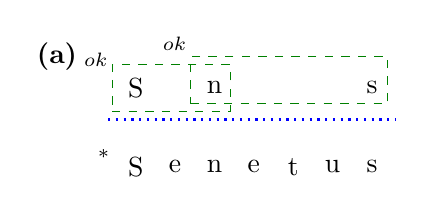
\begin{tikzpicture}
\node (A) at (-1.5,1.4) {\textbf{(a)}};
\node (00) at (-0.9,0.1) {$^{*}$};
\node (0) at (-0.5,0) {\textipa{S}};
\node (0) at (0,0) {e};
\node (1) at (0.5,0) {n};
\node (2) at (1,0) {e};
\node (3) at (1.5,0) {t};
\node (4) at (2,0) {u };
\node (5) at (2.5,0) {s};
%
\node (00) at (-0.5,1) {\textipa{S}};
\node (01) at (0.5,1) {n};
\node (03) at (1.5,1) {};
\node (5) at (2.5,1) {s};
%
\node (000) at (-1,1.3) {$^{ok}$};
\draw [dashed, green!50!black] (-0.8, 0.7) -- (0.7, 0.7) -- (0.7,1.3) -- (-0.8,1.3) -- (-0.8, 0.7);
\node (000) at (0,1.5) {$^{ok}$};
\draw [dashed, green!50!black] (0.2, 0.8) -- (2.7, 0.8) -- (2.7,1.4) -- (0.2,1.4) -- (0.2, 0.8);

\draw[dotted, thick, blue] (-0.85,0.60) to (2.8,0.60);
%   \node at (-0.3,0.40) {{\tiny T}};
    
\end{tikzpicture}
 
        %
    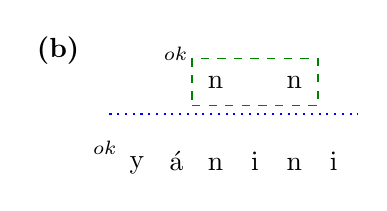
\begin{tikzpicture}
\node (A) at (-1,1.4) {\textbf{(b)}};
\node (00) at (-0.4,0.1) {$^{ok}$};
\node (0) at (0,-0.05) {y};
\node (1) at (0.5,0) {\textipa{\'a}};
\node (2) at (1,-0.05) {n};
\node (3) at (1.5,0) {i};
\node (4) at (2,-0.05) {n};
\node (5) at (2.5,0) {i};
%tier
\node (2) at (1,1) {n};
\node (4) at (2,1) {n};
%
\node (000) at (0.5,1.3) {$^{ok}$};
\draw [dashed, green!50!black] (0.7, 0.7) -- (2.3, 0.7) -- (2.3,1.3) -- (0.7,1.3) -- (0.7, 0.7);

\draw[dotted, thick, blue] (-0.35,0.60) to (2.8,0.60);
%   \node at (-0.3,0.40) {{\tiny T}};
\end{tikzpicture}    
	%
    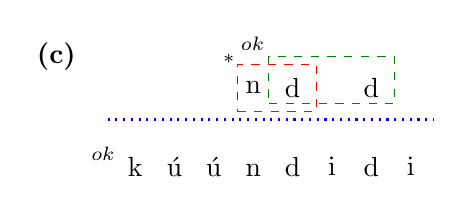
\begin{tikzpicture}
\node (A) at (-1,1.4) {\textbf{(c)}};
\node (00) at (-0.4,0.1) {$^{ok}$};
\node (0) at (0,0) {k};
\node (1) at (0.5,0) {\textipa{\'u}};
\node (2) at (1,0) {\textipa{\'u}};
\node (3) at (1.5,-0.05) {n};
\node (4) at (2,-0) {d};
\node (5) at (2.5,0) {i};
\node (6) at (3,0) {d};
\node (7) at (3.5,0) {i};
%tier
\node (3) at (1.5,1) {n};
\node (4) at (2,1) {d};
\node (6) at (3,1) {d};
%
\node (000) at (1.2,1.3) {$^{*}$};
\draw [dashed, red] (1.3, 0.7) -- (2.3, 0.7) -- (2.3,1.3) -- (1.3,1.3) -- (1.3, 0.7);

\node (000) at (1.5,1.5) {$^{ok}$};
\draw [dashed, green!50!black] (1.7, 0.8) -- (3.3, 0.8) -- (3.3,1.4) -- (1.7,1.4) -- (1.7, 0.8);

\draw[dotted, thick, blue] (-0.35,0.60) to (3.8,0.60);
%   \node at (-0.3,0.40) {{\tiny T}};
\end{tikzpicture}    
        \caption{Example of a TSL analysis of nasal harmony in Yaka: (a) is ill-formed because of tier adjacent $^*$\textipa{[nd]}; (b) is well-formed since  there are no voiced stops on the tier disagreeing in nasality; (c) is well-formed because the \textipa{[d]} immediately following \textipa{[n]} stops the latter from being a trigger for harmony, but it is still ruled out by the constraint needed for (b).}
        \label{fig:YAKA1}
        \end{figure}

The reader might point out that the difference between Fig.~\ref{fig:YAKA1}.a and Fig.~\ref{fig:YAKA1}.c can be resolved by extending the tier-grammar to consider $3$-grams.
However, in order to enforce harmony correctly, the tier-projection places every occurrence of voiced stops in the string on the tier, thus making $3$-grams constraints insufficient (e.g.,Ex.~(\ref{ex:3}c)).
Moreover, since the number of segments between harmonizing elements is potentially unbounded, no TSL grammar can generally account for this pattern, independently of the dimension of the tier $k$-grams.

Let us consider the examples in Ex.~(\ref{ex:3}) once more. 
Any nasal immediately followed by a voiced stop does not trigger harmony. 
In fact, since they do not block the harmonic process, neither the nasal nor the stop participate in the harmony at all.
If we could make the projection of nasals and stops avoid  those segments that appear in specific consonant clusters (e.g.,~\textipa{[nd]}) the tier constraints discussed above would work once again.
This is not possible with TSL as originally defined in \cite{HeinzRawalTanner}, as TSL selects tier elements only based on their $1$-local properties (i.e.,~which kind of segment they are). %Sec.~\ref{sec:SSTSL}.
However, this kind of expressivity can be accomplished by increasing the locality window of the \emph{tier projection mechanism}. 

This is the intuition behind  \citet{desanto2019structure}'s ITSL class: a TSL grammar  can be made simultaneously aware of local and non-local properties of segments in the string with a natural change to the definition of the erasing function.
Fig.~\ref{fig:YAKA2} shows how, by increasing the locality of the projection to $2$, we allow the grammar to project a nasal iff it is not immediately followed by a voiced oral stop, and a voiced stop iff it is not immediately preceded by a nasal.
Then, we can use $2$-local tier constraints to ban  \textipa{[nd]}.
This time,  possible intermediate clusters are not a problem, since the projection is able to infer that they are in local contexts that make them irrelevant to the harmonic process.

\begin{figure}[]
\begin{center}
    %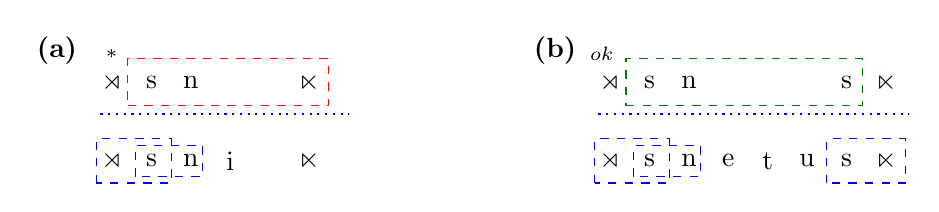
\begin{tikzpicture} %SSTSL EXAMPLE
    \node (A) at (-1.2,1.4) {\textbf{(b)}};
      \node (60) at (-0.5,0) {$\rtimes$};
        \node (0) at (0,0) {s};
        \node (1) at (0.5,0) {n};
        \node (2) at (1,0) {e};
        \node (3) at (1.5,0) {t};
        \node (4) at (2,0) {u };
        \node (5) at (2.5,0) {s};
      \node (6) at (3,0) {$\ltimes$};
        %%tier
             \node (600) at (-0.5,1) {$\rtimes$};
       \node (00) at (0,1) {s};
       \node (01) at (0.5,1) {n};
       \node (5) at (2.5,1) {s};
          \node (06) at (3,1) {$\ltimes$};
        %
        %projection function
       \draw[dashed, blue] (-0.7,-0.28 ) rectangle (0.25, 0.28);
         \draw  [dashed, blue] (-0.2,-0.2 ) rectangle (0.65, 0.2);
         \draw [dashed, blue](2.25,-0.28 ) rectangle (3.25, 0.28);
          %local constraints   
 	 \node (000) at (-0.6,1.3){$^{ok}$};
        \draw [dashed, green!50!black](-0.3, 0.7) -- (2.7, 0.7) -- (2.7,1.3) -- (-0.3,1.3) -- (-0.3, 0.7);
        %tier bar
        \draw[dotted, thick, blue] (-0.65,0.60) to (3.3,0.60);
       % \node at (-0.5,0.40) {{\tiny T}};
        
        \begin{scope}[xshift=-180pt] %string in the center
         \node (A) at (-1.2,1.4) {\textbf{(a)}};
         \node (60) at (-0.5,0) {$\rtimes$};
        \node (0) at (0,0) {s};
        \node (1) at (0.5,0) {n};
        \node (2) at (1,0) {i};
        \node (3) at (1.5,0) {\textglotstop};
         \node (6) at (2,0) {$\ltimes$};
        %%tier
          \node (600) at (-0.5,1) {$\rtimes$};
        \node (00) at (0,1) {s};
        \node (01) at (0.5,1) {n};
          \node (006) at (2,1) {$\ltimes$};
        %projection function
        \draw[dashed, blue] (-0.7,-0.28 ) rectangle (0.25, 0.28);
        \draw  [dashed, blue] (-0.2,-0.2 ) rectangle (0.65, 0.2);
	%local constraints
        \node (000) at (-0.5,1.3) {$^*$};
        \draw [dashed, red] (-0.3, 0.7) -- (2.25, 0.7) -- (2.25,1.3) -- (-0.3,1.3) -- (-0.3, 0.7);
      \draw[dotted, thick, blue] (-0.65,0.60) to (2.5,0.60);
       % \node at (-0.5,0.40) {{\tiny T}};
        %
        \end{scope}
        
        \end{tikzpicture}

     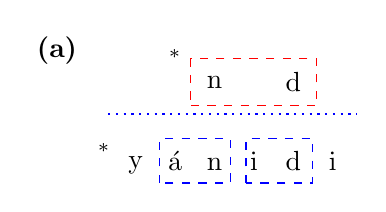
\begin{tikzpicture}

\node (A) at (-1,1.4) {\textbf{(a)}};
\node (00) at (-0.4,0.1) {$^{*}$};
\node (0) at (0,-0.05) {y};
\node (1) at (0.5,0) {\textipa{\'a}};
\node (2) at (1,-0.05) {n};
\node (3) at (1.5,0) {i};
\node (4) at (2,0) {d};
\node (5) at (2.5,0) {i};
%tier
\node (2) at (1,1) {n};
\node (4) at (2,1) {d};
%
\node (000) at (0.5,1.3) {$^{*}$};
\draw [dashed, red] (0.7, 0.7) -- (2.3, 0.7) -- (2.3,1.3) -- (0.7,1.3) -- (0.7, 0.7);
        %projection function
 \draw  [dashed, blue] (0.3,-0.28 ) rectangle (1.2, 0.28);
\draw [dashed, blue](1.4,-0.28 ) rectangle (2.25, 0.28);

\draw[dotted, thick, blue] (-0.35,0.60) to (2.8,0.60);
\end{tikzpicture}
  
    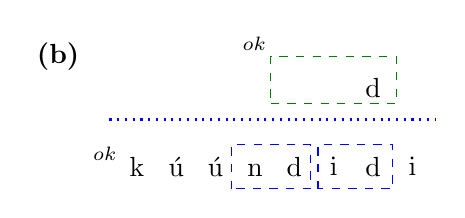
\begin{tikzpicture} %SSTSL EXAMPLE
\node (A) at (-1,1.4) {\textbf{(b)}};
\node (00) at (-0.4,0.1) {$^{ok}$};
\node (0) at (0,0) {k};
\node (1) at (0.5,0) {\textipa{\'u}};
\node (2) at (1,0) {\textipa{\'u}};
\node (3) at (1.5,-0.05) {n};
\node (4) at (2,0) {d};
\node (5) at (2.5,0) {i};
\node (6) at (3,0) {d};
\node (7) at (3.5,0) {i};
%tier
\node (6) at (3,1) {d};
        %
        %projection function
         \draw  [dashed, blue] (1.2,-0.28 ) rectangle (2.2, 0.28);
         \draw [dashed, blue](2.3,-0.28 ) rectangle (3.25, 0.28);
          %local constraints   
\node (000) at (1.5,1.5) {$^{ok}$};
\draw [dashed, green!50!black] (1.7, 0.8) -- (3.3, 0.8) -- (3.3,1.4) -- (1.7,1.4) -- (1.7, 0.8);

        %tier bar
\draw[dotted, thick, blue] (-0.35,0.60) to (3.8,0.60);    
\end{tikzpicture}

      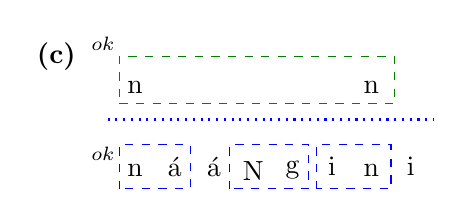
\begin{tikzpicture} %SSTSL EXAMPLE
\node (A) at (-1,1.4) {\textbf{(c)}};
\node (00) at (-0.4,0.1) {$^{ok}$};
\node (0) at (0,-0.05) {n};
\node (1) at (0.5,0) {\textipa{\'a}};
\node (2) at (1,0) {\textipa{\'a}};
\node (3) at (1.5,-0.05) {\textipa{N}};
\node (4) at (2,-0.05) {g};
\node (5) at (2.5,0) {i};
\node (6) at (3,-0.05) {n};
\node (7) at (3.5,0) {i};
%tier
\node (0) at (0,1) {n};
\node (6) at (3,1) {n};
        %
        %projection function
         \draw  [dashed, blue] (-0.2,-0.28 ) rectangle (0.7, 0.28);
         \draw  [dashed, blue] (1.2,-0.28 ) rectangle (2.2, 0.28);
         \draw [dashed, blue](2.3,-0.28 ) rectangle (3.25, 0.28);
          %local constraints   
\node (000) at (-0.4,1.5) {$^{ok}$};
\draw [dashed, green!50!black] (-0.2, 0.8) -- (3.3, 0.8) -- (3.3,1.4) -- (-0.2,1.4) -- (-0.2, 0.8);

        %tier bar
\draw[dotted, thick, blue] (-0.35,0.60) to (3.8,0.60);    
\end{tikzpicture}


        \end{center}
        % \caption{Example from Samala, allowing generalized tier projection: (a) is ill-formed because of $^*$\textipa{sn}; (b) is well-formed since  \textipa{[sn]} is followed by \textipa{[s]} later in the string. Note that \textipa{[n]} is projected on the tier only when adjacent to \textipa{[s]}.}
         %if changed to new fig
        \caption{Example of a ITSL analysis of nasal harmony in Yaka: (a) is ill-formed because of adjacent $^*$\textipa{[nd]}; (b) is well-formed since  \textipa{[n]} is followed by another  \textipa{[n]} later in the string; (c) is well-formed because the \textipa{[nd]} cluster does not enforce nasality on the following stops.  Note that \textipa{[n,d,g,N]} are projected on the tier only when not immediately adjacent in the input. }
        \label{fig:YAKA2}
        \end{figure}

ITSL languages have been shown to properly extend TSL, and fix a gap in its typological coverage. 
However, there is a second shortcoming to adopting TSL as a model for natural language phonotactics, that carries over to ITSL:  TSL (and thus ITSL) languages are not closed under intersection.

Lack of closure under intersection is problematic as it entails that the complexity of phonological dependencies is no longer constant under factorization.
This implies that the upper bound for phonological phenomena would shift, depending on whether one treats a constraint as a single phenomenon or the interaction of multiple phenomena.
Moreover, we clearly want to be able to consider multiple phenomena at the same time when describing the phonotactics of a language.
Consider the following additional data from Yaka.


\begin{exe}
    \ex\label{ex:4}\begin{xlist}
    	 \ex\label{ex:4a} \textipa{k\'em-ene}   
	 \ex\label{ex:4b} \textipa{k\'eb-ede}
	\end{xlist}
\end{exe}

Ex.~(\ref{ex:4}) shows a vowel alternation that is independent of the nasality process, and is instead due to vowel heigh harmony.
Vowel harmony can be easily accounted for with a TSL grammar.
However, this is only true if we analyze it by itself, and fails if we try to model nasal harmony and vowel harmony in a single grammar.
In order to account for this, vowels would need to be projected on the tier, thus interfering with the nasalization process.
To account for this, \citet{desanto2019structure} propose  working with the intersection closure of TSL (MTSL) and ITSL languages (MITSL).

Intuitively, MTSL and MITSL can be conceptualized as encoding multiple projections (tiers) at the same time, and enforcing independent strictly local constraints over each tier.
For a string to belong to the language, it needs to be well-formed on every tier.
For instance, Fig.~\ref{fig:YAKA3} shows a grammar projecting two separate tier: a tier of vowel, with constraints ensuring height harmony; and a tier enforcing nasal harmony as in the examples above.


\begin{figure}[]
\begin{center}
    %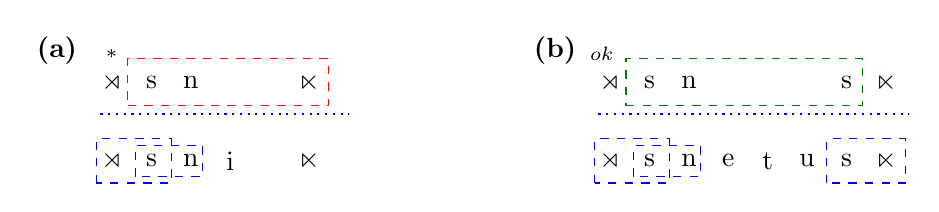
\begin{tikzpicture} %SSTSL EXAMPLE
    \node (A) at (-1.2,1.4) {\textbf{(b)}};
      \node (60) at (-0.5,0) {$\rtimes$};
        \node (0) at (0,0) {s};
        \node (1) at (0.5,0) {n};
        \node (2) at (1,0) {e};
        \node (3) at (1.5,0) {t};
        \node (4) at (2,0) {u };
        \node (5) at (2.5,0) {s};
      \node (6) at (3,0) {$\ltimes$};
        %%tier
             \node (600) at (-0.5,1) {$\rtimes$};
       \node (00) at (0,1) {s};
       \node (01) at (0.5,1) {n};
       \node (5) at (2.5,1) {s};
          \node (06) at (3,1) {$\ltimes$};
        %
        %projection function
       \draw[dashed, blue] (-0.7,-0.28 ) rectangle (0.25, 0.28);
         \draw  [dashed, blue] (-0.2,-0.2 ) rectangle (0.65, 0.2);
         \draw [dashed, blue](2.25,-0.28 ) rectangle (3.25, 0.28);
          %local constraints   
 	 \node (000) at (-0.6,1.3){$^{ok}$};
        \draw [dashed, green!50!black](-0.3, 0.7) -- (2.7, 0.7) -- (2.7,1.3) -- (-0.3,1.3) -- (-0.3, 0.7);
        %tier bar
        \draw[dotted, thick, blue] (-0.65,0.60) to (3.3,0.60);
       % \node at (-0.5,0.40) {{\tiny T}};
        
        \begin{scope}[xshift=-180pt] %string in the center
         \node (A) at (-1.2,1.4) {\textbf{(a)}};
         \node (60) at (-0.5,0) {$\rtimes$};
        \node (0) at (0,0) {s};
        \node (1) at (0.5,0) {n};
        \node (2) at (1,0) {i};
        \node (3) at (1.5,0) {\textglotstop};
         \node (6) at (2,0) {$\ltimes$};
        %%tier
          \node (600) at (-0.5,1) {$\rtimes$};
        \node (00) at (0,1) {s};
        \node (01) at (0.5,1) {n};
          \node (006) at (2,1) {$\ltimes$};
        %projection function
        \draw[dashed, blue] (-0.7,-0.28 ) rectangle (0.25, 0.28);
        \draw  [dashed, blue] (-0.2,-0.2 ) rectangle (0.65, 0.2);
	%local constraints
        \node (000) at (-0.5,1.3) {$^*$};
        \draw [dashed, red] (-0.3, 0.7) -- (2.25, 0.7) -- (2.25,1.3) -- (-0.3,1.3) -- (-0.3, 0.7);
      \draw[dotted, thick, blue] (-0.65,0.60) to (2.5,0.60);
       % \node at (-0.5,0.40) {{\tiny T}};
        %
        \end{scope}
        
        \end{tikzpicture}

     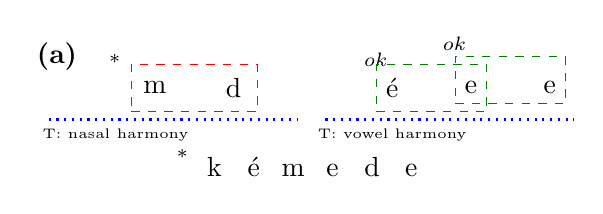
\begin{tikzpicture}

\node (A) at (-2,1.4) {\textbf{(a)}};
\node (00) at (-0.4,0.1) {$^{*}$};
\node (0) at (0,0) {k};
\node (1) at (0.5,0) {\textipa{\'e}};
\node (2) at (1,-0.05) {m};
\node (3) at (1.5,-0.05) {e};
\node (4) at (2,0) {d};
\node (5) at (2.5,-0.05) {e};
        %projection function
% \draw  [dashed, blue] (0.3,-0.28 ) rectangle (1.2, 0.28);
%\draw [dashed, blue](1.4,-0.28 ) rectangle (2.25, 0.28);
%%
\begin{scope}[xshift=50pt]
\node (1) at (0.5,1) {\textipa{\'e}};
\node (3) at (1.5,1) {e};
\node (5) at (2.5,1) {e};
%
\node (000) at (0.3,1.3) {$^{ok}$};
\draw [dashed, green!50!black] (0.3, 0.7) -- (1.7, 0.7) -- (1.7,1.3) -- (0.3,1.3) -- (0.3, 0.7);
\node (000) at (1.3,1.5) {$^{ok}$};
\draw [dashed, green!50!black] (1.3, 0.8) -- (2.7, 0.8) -- (2.7,1.4) -- (1.3,1.4) -- (1.3, 0.8);
\draw[dotted, thick, blue] (-0.35,0.60) to (2.8,0.60);
\node at (0.5,0.40) {{\tiny T: vowel harmony}};
\end{scope}
\begin{scope}[xshift=-50pt]
\node (2) at (1,1) {m};
\node (4) at (2,1) {d};
%
\node (000) at (0.5,1.3) {$^{*}$};
\draw [dashed, red] (0.7, 0.7) -- (2.3, 0.7) -- (2.3,1.3) -- (0.7,1.3) -- (0.7, 0.7);
\draw[dotted, thick, blue] (-0.35,0.60) to (2.8,0.60);
\node at (0.5,0.40) {{\tiny T: nasal harmony}};
\end{scope}
\end{tikzpicture}
  
    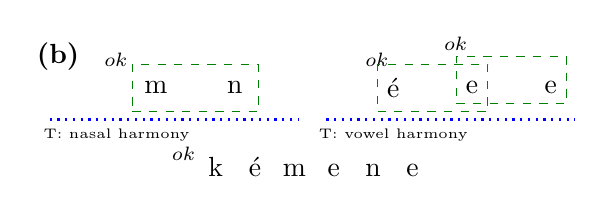
\begin{tikzpicture}

\node (A) at (-2,1.4) {\textbf{(b)}};
\node (00) at (-0.4,0.1) {$^{ok}$};
\node (0) at (0,0) {k};
\node (1) at (0.5,0) {\textipa{\'e}};
\node (2) at (1,-0.05) {m};
\node (3) at (1.5,-0.05) {e};
\node (4) at (2,-0.05) {n};
\node (5) at (2.5,-0.05) {e};
        %projection function
% \draw  [dashed, blue] (0.3,-0.28 ) rectangle (1.2, 0.28);
%\draw [dashed, blue](1.4,-0.28 ) rectangle (2.25, 0.28);
%%
\begin{scope}[xshift=50pt]
\node (1) at (0.5,1) {\textipa{\'e}};
\node (3) at (1.5,1) {e};
\node (5) at (2.5,1) {e};
%
\node (000) at (0.3,1.3) {$^{ok}$};
\draw [dashed, green!50!black] (0.3, 0.7) -- (1.7, 0.7) -- (1.7,1.3) -- (0.3,1.3) -- (0.3, 0.7);
\node (000) at (1.3,1.5) {$^{ok}$};
\draw [dashed, green!50!black] (1.3, 0.8) -- (2.7, 0.8) -- (2.7,1.4) -- (1.3,1.4) -- (1.3, 0.8);
\draw[dotted, thick, blue] (-0.35,0.60) to (2.8,0.60);
\node at (0.5,0.40) {{\tiny T: vowel harmony}};
\end{scope}
\begin{scope}[xshift=-50pt]
\node (2) at (1,1) {m};
\node (4) at (2,1) {n};
%
\node (000) at (0.5,1.3) {$^{ok}$};
\draw [dashed,  green!50!black] (0.7, 0.7) -- (2.3, 0.7) -- (2.3,1.3) -- (0.7,1.3) -- (0.7, 0.7);
\draw[dotted, thick, blue] (-0.35,0.60) to (2.8,0.60);
\node at (0.5,0.40) {{\tiny T: nasal harmony}};
\end{scope}
\end{tikzpicture}

        \end{center}
        % \caption{Example from Samala, allowing generalized tier projection: (a) is ill-formed because of $^*$\textipa{sn}; (b) is well-formed since  \textipa{[sn]} is followed by \textipa{[s]} later in the string. Note that \textipa{[n]} is projected on the tier only when adjacent to \textipa{[s]}.}
         %if changed to new fig
        \caption{Example of a MITSL analysis of  Yaka nasal and vowel harmony: (a) is ill-formed because there is a violation on the nasal harmony tier; (b) is well-formed since there are no violations on either tier.}
        \label{fig:YAKA3}
        \end{figure}


Since intersection closure is a fundamentally desirable property from a linguistic perspective, \citet{McMullinSCIL2019} propose an algorithm that efficiently learns multiple tier-based strictly $2$-local  (i.e.,~where tier constraints are bigrams) dependencies, with no a-priori knowledge about the tier-segments or the number of tiers required.
Given the typological importance of input-sensitive projection, in this paper we expand on \citet{McMullinSCIL2019} and present a grammatical inference algorithm able to learn MITSL grammars with $2$-local contexts and $2$-local tier constraints ($k$-MITSL$^2_2$), only from positive examples and without a-priori knowledge about the content --- or the number --- of necessary tiers.
Moreover, since MTSL languages are properly contained in MITSL, we also implicitly provide an implementation of  \citet{McMullinSCIL2019}'s approach.


%Many dependencies in phonology can be captured by strictly local (SL) grammars: \emph{local constraints} that only make distinctions on the basis of contiguous substrings of segments up to some length $k$ \citep[essentially, $k$-grams;][]{Heinz2011a}.
%For example, a ($k$=2) local dependency requiring \textipa{/s/} to surface as \textipa{[z]} when followed by \textipa{[l]} can be captured by a grammar that forbids the sequence \textipa{[sl]}.
%However, while prominent in natural language phonology, (unbounded) long-distance dependencies cannot be captured by local constraints.
%To account for this, work studying linguistic dependencies from a formal language theoretical perspective has characterized long-distance phonotactic patterns  as \emph{tier-based strictly local}.
%%We give a full introduction to the mathematical properties of TSL in Section~\ref{ssec:Subreg_intro}, but an informal treatment will suffice for now.
%
%Tier-based strictly local languages (TSL) are able to encode a notion of relativized locality inspired by the idea of phonological tier, already popular in autosegmental phonology   \cite{goldsmith1976autosegmental}.
%While a  formal introduction  to the properties of TSL  is beyond the scope of this paper,  a TSL dependency is intuitively non-local in the input string but local over a \emph{tier}.
%A tier is defined as the projection of a subset of the segments of the input string, and the grammar constraints are characterized as the set of sequences of length $k$ not allowed on the tier.
%For instance, the example in Figure~\ref{fig:Aari} (from Aari, an Omotic language of south Ethiopia) shows how to enforce long-distance sibilant harmony in anteriority.
%First one projects from the string a tier $T$ that only contains sibilants, and then one bans contiguous \textipa{[\textctyogh s]} and \textipa{[s\textctyogh]} on $T$  \cite[see][]{Hayward_Aari}.
%%
% \begin{figure}[h!]
%\begin{center}
%%\resizebox{0.6\textwidth}{!}{%
%\begin{tikzpicture}
 \node (00) at (-0.4,0.1) {$^{*}$};
\node (0) at (0,0) {\textyogh };
\node (1) at (0.5,0) {a:};
\node (2) at (1,0) {e};
\node (3) at (1.5,0) {r};
\node (4) at (2,0) {s};
\node (5) at (2.5,0) {e};
%tier
\node (000) at (-0.4,1.3) {$^*$};
\node (00) at (0,1) {\textyogh };
\node (05) at (2,1) {s};

\draw [dashed, red] (-0.3, 0.7) -- (2.2, 0.7) -- (2.2,1.3) -- (-0.3,1.3) -- (-0.3, 0.7);

\draw[dotted, thick, blue] (-0.35,0.55) to (2.8,0.55);
%\node at (0.5,0.40) {{\tiny T: sibilant harmony}};

\begin{scope}[xshift=120pt]
 \node (00) at (-0.4,0.1) {$^{ok}$};
\node (0) at (0,0) {\textyogh };
\node (1) at (0.5,0) {a:};
\node (2) at (1,0) {e};
\node (3) at (1.5,0) {r};
\node (4) at (2,0) {\textesh };
\node (5) at (2.5,0) {e};
%tier
\node (000) at (-0.5,1.3) {$^{ok}$};
\node (00) at (0,1) {\textyogh };
\node (05) at (2,1) {\textesh };

\draw [dashed, green!50!black] (-0.3, 0.7) -- (2.2, 0.7) -- (2.2,1.3) -- (-0.3,1.3) -- (-0.3, 0.7);
\draw[dotted, thick, blue] (-0.35,0.55) to (2.8,0.55);
%\node at (0.5,0.40) {{\tiny T: sibilant harmony}};
\end{scope}

\end{tikzpicture}

%%}
%\end{center}
%\caption{Example of sibilant harmony over tier from Aari. }
%\label{fig:Aari}
%\end{figure}
%%\vspace{-0.3cm}
%
%The class of TSL languages has been shown to have good cross-linguistic coverage, accounting for a variety of different phonotactic patters cross-linguistically \citep{HeinzRawalTanner,McMullin16,Graf17Phonology}.
%Moreover, and most interesting to us, TSL$_k$ languages have been shown to be efficiently (polynomial in time and input) learnable in the limit from positive data, even when the tier-alphabet is not known \emph{a priori}  \citep{JardineHeinz16,jardinemcmullin17}.
%
%However, there are two main known limits to TSL as a good formal account for natural language phonotactics.
%
%First, it is known that TSL languages are not closed under intersection.
%Lack of closure under intersection is problematic as it entails that the complexity of phonological dependencies is no longer constant under factorization.
%This implies that the upper bound for phonological phenomena would shift, depending on whether one treats a constraint as a single phenomenon or the interaction of multiple phenomena.
%Moreover, we clearly want to be able to consider multiple phenomena at the same time when describing the phonotactics of a language.
%Intersection closure is thus a fundamentally desirable property from a linguistic perspective.
%To account for this, \citet{desanto2019structure} propose the multiple tier-based strictly local (MTSL) class, as a proper extension of TSL formalizing its intersection closure.
%Intuitively, MTSL can be conceptualized has a class encoding multiple projections (tiers) at the same time, and enforcing distinct strictly local constraints over each tier.
%\citet{McMullinSCIL2019} propose an algorithm that efficiently learns multiple tier-based strictly $2$-local  (i.e. where tier constraints are bigrams) dependencies, with no a-priori knowledge about the tier-segments or the number of tiers required.
%
%
%The second limit of TSL lies in the simplicity of its projection mechanism.
%Recently, several patterns have been reported that cannot be described by the way TSL currently uses tier projection to mask out parts of a string before enforcing some strictly local constraint \citep{McMullin16,MayerMajor18,Baek2017CLS,graf2018sanskrit,desanto2019structure}.
%These patterns include the long-distance sibilant harmony in Imdlawn Tashlhiyt  \citep{McMullin16}, the nasal harmony pattern in Yaka \cite{WalkerYaka}, the unbounded stress of Classical Arabic (see \cite{Baek2017CLS} and references therein), and cases of unbounded tone plateauing.
%These patterns share the common trait that one has to inspect the local context of a segment before projecting it on a tier. 
%
%Consider the case of Consonantal Nasal harmony in Yaka, in which a nasal stop induces nasalization of voiced consonants occurring at any distance to its right  \cite{hyman1995nasal,Walker_Yaka}.
%For instance, the  segmental alternation shown in  Ex.~(\ref{ex:1}) is due to the phoneme \textipa{/d/} surfacing as  \textipa{[n]} after a preceding nasal  (cf.  Ex.~(\ref{ex:1a}, \ref{ex:1b} vs.  \ref{ex:1c})).\@
%Vowels and voiceless consonants intervening between the two harmonizing stops remain unaffected  (cf. Ex.~(\ref{ex:2})).
%
%
%\begin{exe}
%    \ex\label{ex:1}\begin{xlist}
%    	 \ex\label{ex:1a} \textipa{y\'an-ini}   `\emph{to cry out}'
%	 \ex\label{ex:1b} \textipa{y\'ad-idi}   `\emph{to spread}'
%	 \ex\label{ex:1c} $^*$\textipa{y\'an-idi}      
%	\end{xlist}
%    \ex\label{ex:2}\begin{xlist}
%     	\ex\label{ex:2a}\textipa{h\'am\'uk-ini} `\emph{to give away}'
%    	\ex\label{ex:2b}\textipa{m\'i\'ituk-ini} `\emph{to sulk}'
%    \end{xlist}
%     \ex\label{ex:3}\begin{xlist}
%    	 \ex\label{ex:3a}    \textipa{b\'i\'imb-idi} `\emph{to embrace}'
%	 \ex\label{ex:3b}  \textipa{k\'u\'und-idi} `\emph{to bury}'
%	 \ex\label{ex:3c}  \textipa{n\'a\'aNg-ini} `\emph{to last}'
%	\end{xlist}
%\end{exe}
%
%A TSL analysis for this patter seems straightforward, as this data can be captured by projecting a tier of voiced consonants, and enforcing constraints banning tier adjacent  \textipa{[nd]}.
%
%\begin{figure}[t]
%\centering
%    \begin{tikzpicture}

\node (A) at (-1,1.4) {\textbf{(a)}};
\node (00) at (-0.4,0.1) {$^{*}$};
\node (0) at (0,-0.05) {y};
\node (1) at (0.5,0) {\textipa{\'a}};
\node (2) at (1,-0.05) {n};
\node (3) at (1.5,0) {i};
\node (4) at (2,0) {d};
\node (5) at (2.5,0) {i};
%tier
\node (2) at (1,1) {n};
\node (4) at (2,1) {d};
%
\node (000) at (0.5,1.3) {$^{*}$};
\draw [dashed, red] (0.7, 0.7) -- (2.3, 0.7) -- (2.3,1.3) -- (0.7,1.3) -- (0.7, 0.7);

\draw[dotted, thick, blue] (-0.35,0.60) to (2.8,0.60);
%   \node at (-0.3,0.40) {{\tiny T}};
\begin{scope}[xshift=150pt]
\node (A) at (-1,1.4) {\textbf{(b)}};
\node (00) at (-0.4,0.1) {$^{ok}$};
\node (0) at (0,-0.05) {y};
\node (1) at (0.5,0) {\textipa{\'a}};
\node (2) at (1,-0.05) {n};
\node (3) at (1.5,0) {i};
\node (4) at (2,-0.05) {n};
\node (5) at (2.5,0) {i};
%tier
\node (2) at (1,1) {n};
\node (4) at (2,1) {n};
%
\node (000) at (0.5,1.3) {$^{ok}$};
\draw [dashed, green!50!black] (0.7, 0.7) -- (2.3, 0.7) -- (2.3,1.3) -- (0.7,1.3) -- (0.7, 0.7);

\draw[dotted, thick, blue] (-0.35,0.60) to (2.8,0.60);
%   \node at (-0.3,0.40) {{\tiny T}};
\end{scope}
\end{tikzpicture}
   %    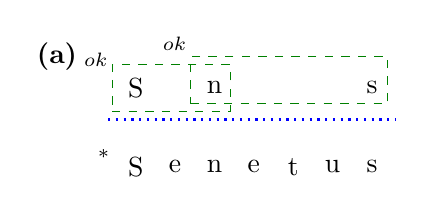
\begin{tikzpicture}
\node (A) at (-1.5,1.4) {\textbf{(a)}};
\node (00) at (-0.9,0.1) {$^{*}$};
\node (0) at (-0.5,0) {\textipa{S}};
\node (0) at (0,0) {e};
\node (1) at (0.5,0) {n};
\node (2) at (1,0) {e};
\node (3) at (1.5,0) {t};
\node (4) at (2,0) {u };
\node (5) at (2.5,0) {s};
%
\node (00) at (-0.5,1) {\textipa{S}};
\node (01) at (0.5,1) {n};
\node (03) at (1.5,1) {};
\node (5) at (2.5,1) {s};
%
\node (000) at (-1,1.3) {$^{ok}$};
\draw [dashed, green!50!black] (-0.8, 0.7) -- (0.7, 0.7) -- (0.7,1.3) -- (-0.8,1.3) -- (-0.8, 0.7);
\node (000) at (0,1.5) {$^{ok}$};
\draw [dashed, green!50!black] (0.2, 0.8) -- (2.7, 0.8) -- (2.7,1.4) -- (0.2,1.4) -- (0.2, 0.8);

\draw[dotted, thick, blue] (-0.85,0.60) to (2.8,0.60);
%   \node at (-0.3,0.40) {{\tiny T}};
    
\end{tikzpicture}
 
%        %
%    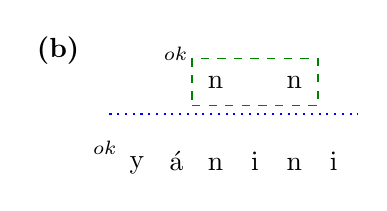
\begin{tikzpicture}
\node (A) at (-1,1.4) {\textbf{(b)}};
\node (00) at (-0.4,0.1) {$^{ok}$};
\node (0) at (0,-0.05) {y};
\node (1) at (0.5,0) {\textipa{\'a}};
\node (2) at (1,-0.05) {n};
\node (3) at (1.5,0) {i};
\node (4) at (2,-0.05) {n};
\node (5) at (2.5,0) {i};
%tier
\node (2) at (1,1) {n};
\node (4) at (2,1) {n};
%
\node (000) at (0.5,1.3) {$^{ok}$};
\draw [dashed, green!50!black] (0.7, 0.7) -- (2.3, 0.7) -- (2.3,1.3) -- (0.7,1.3) -- (0.7, 0.7);

\draw[dotted, thick, blue] (-0.35,0.60) to (2.8,0.60);
%   \node at (-0.3,0.40) {{\tiny T}};
\end{tikzpicture}    
%	%
%    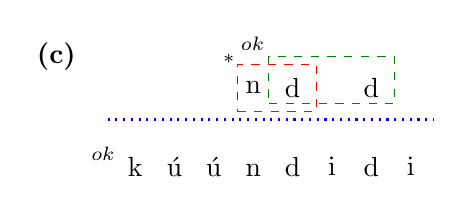
\begin{tikzpicture}
\node (A) at (-1,1.4) {\textbf{(c)}};
\node (00) at (-0.4,0.1) {$^{ok}$};
\node (0) at (0,0) {k};
\node (1) at (0.5,0) {\textipa{\'u}};
\node (2) at (1,0) {\textipa{\'u}};
\node (3) at (1.5,-0.05) {n};
\node (4) at (2,-0) {d};
\node (5) at (2.5,0) {i};
\node (6) at (3,0) {d};
\node (7) at (3.5,0) {i};
%tier
\node (3) at (1.5,1) {n};
\node (4) at (2,1) {d};
\node (6) at (3,1) {d};
%
\node (000) at (1.2,1.3) {$^{*}$};
\draw [dashed, red] (1.3, 0.7) -- (2.3, 0.7) -- (2.3,1.3) -- (1.3,1.3) -- (1.3, 0.7);

\node (000) at (1.5,1.5) {$^{ok}$};
\draw [dashed, green!50!black] (1.7, 0.8) -- (3.3, 0.8) -- (3.3,1.4) -- (1.7,1.4) -- (1.7, 0.8);

\draw[dotted, thick, blue] (-0.35,0.60) to (3.8,0.60);
%   \node at (-0.3,0.40) {{\tiny T}};
\end{tikzpicture}    
%        \caption{Example of a TSL analysis of nasal harmony in Yaka: (a) is ill-formed because of tier adjacent $^*$\textipa{[nd]}; (b) is well-formed since  there are no voiced stops on the tier disagreeing in nasality; (c) is well-formed because the \textipa{[d]} immediately following \textipa{[n]} stops the latter from being a trigger for harmony, but it is still ruled out by the constraint needed for (b).}
%        \label{fig:YAKA1}
%        \end{figure}
%
%
%
%However, observe now the examples in  Ex.~(\ref{ex:3}): consonantal complexes composed of a nasal and a voiced oral stop neither trigger   Ex.~(\ref{ex:3a},\ref{ex:3b}) nor block nasality agreement   Ex.~(\ref{ex:3c}).
%Fig.~\ref{fig:YAKA1} exemplifies why this interaction of a local and a non-local dependency is not TSL\@. 
%Since \textipa{[nd]} is sometimes observed in a string-adjacent context (as in Ex.~(\ref{ex:3b})), it must be permitted as a $2$-gram on a tier --- even though it is only allowed when  \textipa{[nd]} re immediately adjacent in the string.
%But then,  a TSL grammar would have no means of distinguishing Ex.~(\ref{ex:1b}) from Ex.~(\ref{ex:3b}).
%
%The reader might point out that the difference between Fig.~\ref{fig:YAKA1}.a and Fig.~\ref{fig:YAKA1}.c can be resolved by extending the tier-grammar to consider $3$-grams.
%However, in order to enforce harmony correctly, the tier-projection places every occurrence of voiced stops in the string on the tier, thus making $3$-grams constraints insufficient (e.g., Ex.~(\ref{ex:3}c)).
%Moreover, since the number of segments between harmonizing elements is potentially unbounded, no TSL grammar can generally account for this pattern, independently of the dimension of the tier $k$-grams.
%
%Let us consider the examples in Ex.~(\ref{ex:3}) once more. 
%Any nasal immediately followed by a voiced stop does not trigger harmony. 
%In fact, since they do not block the harmonic process, neither the nasal nor the stop participate in the harmony at all.
%If we could make the projection of nasals and stops avoid  those segments that appear in specific consonant clusters (e.g. \textipa{[nd]}) the tier constraints discussed above would work once again.
%This is not possible with TSL as originally defined in \cite{HeinzRawalTanner}, as TSL selects tier elements only based on their $1$-local properties (i.e. which kind of segment they are). %Sec.~\ref{sec:SSTSL}.
%However, this kind of expressivity can be accomplished by increasing the locality window of the \emph{tier projection mechanism}. 
%
%In particular, the intuition behind  \citet{desanto2019structure}'s ITSL class is that  a TSL grammar  can be made simultaneously aware of local and non-local properties of segments in the string with a natural change to the definition of the erasing function.
%
%\begin{figure}[]
%\begin{center}
%    %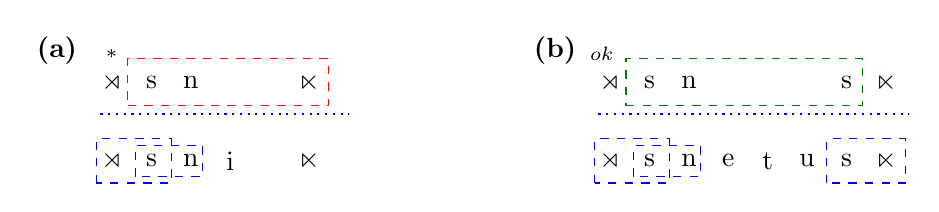
\begin{tikzpicture} %SSTSL EXAMPLE
    \node (A) at (-1.2,1.4) {\textbf{(b)}};
      \node (60) at (-0.5,0) {$\rtimes$};
        \node (0) at (0,0) {s};
        \node (1) at (0.5,0) {n};
        \node (2) at (1,0) {e};
        \node (3) at (1.5,0) {t};
        \node (4) at (2,0) {u };
        \node (5) at (2.5,0) {s};
      \node (6) at (3,0) {$\ltimes$};
        %%tier
             \node (600) at (-0.5,1) {$\rtimes$};
       \node (00) at (0,1) {s};
       \node (01) at (0.5,1) {n};
       \node (5) at (2.5,1) {s};
          \node (06) at (3,1) {$\ltimes$};
        %
        %projection function
       \draw[dashed, blue] (-0.7,-0.28 ) rectangle (0.25, 0.28);
         \draw  [dashed, blue] (-0.2,-0.2 ) rectangle (0.65, 0.2);
         \draw [dashed, blue](2.25,-0.28 ) rectangle (3.25, 0.28);
          %local constraints   
 	 \node (000) at (-0.6,1.3){$^{ok}$};
        \draw [dashed, green!50!black](-0.3, 0.7) -- (2.7, 0.7) -- (2.7,1.3) -- (-0.3,1.3) -- (-0.3, 0.7);
        %tier bar
        \draw[dotted, thick, blue] (-0.65,0.60) to (3.3,0.60);
       % \node at (-0.5,0.40) {{\tiny T}};
        
        \begin{scope}[xshift=-180pt] %string in the center
         \node (A) at (-1.2,1.4) {\textbf{(a)}};
         \node (60) at (-0.5,0) {$\rtimes$};
        \node (0) at (0,0) {s};
        \node (1) at (0.5,0) {n};
        \node (2) at (1,0) {i};
        \node (3) at (1.5,0) {\textglotstop};
         \node (6) at (2,0) {$\ltimes$};
        %%tier
          \node (600) at (-0.5,1) {$\rtimes$};
        \node (00) at (0,1) {s};
        \node (01) at (0.5,1) {n};
          \node (006) at (2,1) {$\ltimes$};
        %projection function
        \draw[dashed, blue] (-0.7,-0.28 ) rectangle (0.25, 0.28);
        \draw  [dashed, blue] (-0.2,-0.2 ) rectangle (0.65, 0.2);
	%local constraints
        \node (000) at (-0.5,1.3) {$^*$};
        \draw [dashed, red] (-0.3, 0.7) -- (2.25, 0.7) -- (2.25,1.3) -- (-0.3,1.3) -- (-0.3, 0.7);
      \draw[dotted, thick, blue] (-0.65,0.60) to (2.5,0.60);
       % \node at (-0.5,0.40) {{\tiny T}};
        %
        \end{scope}
        
        \end{tikzpicture}

%     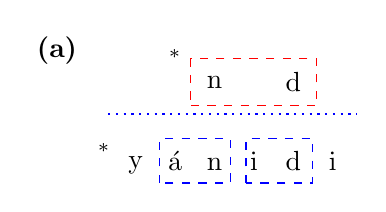
\begin{tikzpicture}

\node (A) at (-1,1.4) {\textbf{(a)}};
\node (00) at (-0.4,0.1) {$^{*}$};
\node (0) at (0,-0.05) {y};
\node (1) at (0.5,0) {\textipa{\'a}};
\node (2) at (1,-0.05) {n};
\node (3) at (1.5,0) {i};
\node (4) at (2,0) {d};
\node (5) at (2.5,0) {i};
%tier
\node (2) at (1,1) {n};
\node (4) at (2,1) {d};
%
\node (000) at (0.5,1.3) {$^{*}$};
\draw [dashed, red] (0.7, 0.7) -- (2.3, 0.7) -- (2.3,1.3) -- (0.7,1.3) -- (0.7, 0.7);
        %projection function
 \draw  [dashed, blue] (0.3,-0.28 ) rectangle (1.2, 0.28);
\draw [dashed, blue](1.4,-0.28 ) rectangle (2.25, 0.28);

\draw[dotted, thick, blue] (-0.35,0.60) to (2.8,0.60);
\end{tikzpicture}
  
%    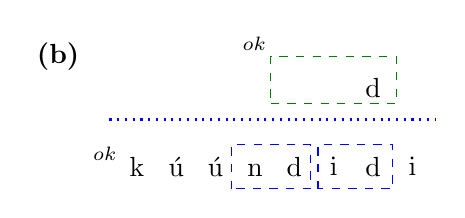
\begin{tikzpicture} %SSTSL EXAMPLE
\node (A) at (-1,1.4) {\textbf{(b)}};
\node (00) at (-0.4,0.1) {$^{ok}$};
\node (0) at (0,0) {k};
\node (1) at (0.5,0) {\textipa{\'u}};
\node (2) at (1,0) {\textipa{\'u}};
\node (3) at (1.5,-0.05) {n};
\node (4) at (2,0) {d};
\node (5) at (2.5,0) {i};
\node (6) at (3,0) {d};
\node (7) at (3.5,0) {i};
%tier
\node (6) at (3,1) {d};
        %
        %projection function
         \draw  [dashed, blue] (1.2,-0.28 ) rectangle (2.2, 0.28);
         \draw [dashed, blue](2.3,-0.28 ) rectangle (3.25, 0.28);
          %local constraints   
\node (000) at (1.5,1.5) {$^{ok}$};
\draw [dashed, green!50!black] (1.7, 0.8) -- (3.3, 0.8) -- (3.3,1.4) -- (1.7,1.4) -- (1.7, 0.8);

        %tier bar
\draw[dotted, thick, blue] (-0.35,0.60) to (3.8,0.60);    
\end{tikzpicture}

%      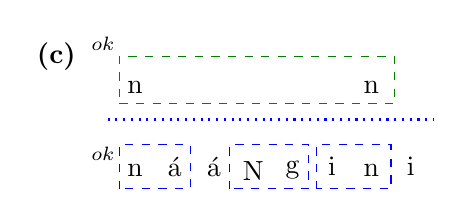
\begin{tikzpicture} %SSTSL EXAMPLE
\node (A) at (-1,1.4) {\textbf{(c)}};
\node (00) at (-0.4,0.1) {$^{ok}$};
\node (0) at (0,-0.05) {n};
\node (1) at (0.5,0) {\textipa{\'a}};
\node (2) at (1,0) {\textipa{\'a}};
\node (3) at (1.5,-0.05) {\textipa{N}};
\node (4) at (2,-0.05) {g};
\node (5) at (2.5,0) {i};
\node (6) at (3,-0.05) {n};
\node (7) at (3.5,0) {i};
%tier
\node (0) at (0,1) {n};
\node (6) at (3,1) {n};
        %
        %projection function
         \draw  [dashed, blue] (-0.2,-0.28 ) rectangle (0.7, 0.28);
         \draw  [dashed, blue] (1.2,-0.28 ) rectangle (2.2, 0.28);
         \draw [dashed, blue](2.3,-0.28 ) rectangle (3.25, 0.28);
          %local constraints   
\node (000) at (-0.4,1.5) {$^{ok}$};
\draw [dashed, green!50!black] (-0.2, 0.8) -- (3.3, 0.8) -- (3.3,1.4) -- (-0.2,1.4) -- (-0.2, 0.8);

        %tier bar
\draw[dotted, thick, blue] (-0.35,0.60) to (3.8,0.60);    
\end{tikzpicture}


%        \end{center}
%        % \caption{Example from Samala, allowing generalized tier projection: (a) is ill-formed because of $^*$\textipa{sn}; (b) is well-formed since  \textipa{[sn]} is followed by \textipa{[s]} later in the string. Note that \textipa{[n]} is projected on the tier only when adjacent to \textipa{[s]}.}
%         %if changed to new fig
%        \caption{Example of a ITSL analysis of nasal harmony in Yaka: (a) is ill-formed because of adjacent $^*$\textipa{[nd]}; (b) is well-formed since  \textipa{[n]} is followed by another  \textipa{[n]} later in the string; (c) is well-formed because the \textipa{[nd]} cluster does not enforce nasality on the following stops.  Note that \textipa{[n,d]} are projected on the tier only when not immediately adjacent in the input. }
%        \label{fig:YAKA2}
%        \end{figure}
%
%
%Fig.~\ref{fig:YAKA2} shows how, by increasing the locality of the projection to $2$, we allow the grammar to project a nasal iff it is not immediately followed by a voiced oral stop, and then use $2$-local tier constraints to ban  \textipa{nd}.%
%This time,  possible intermediate clusters are not a problem, since the projection is able to infer that they are in local contexts that make them irrelevant to the harmonic process.
%
%Finally, note the following additional data:
%
%
%\begin{exe}
%    \ex\label{ex:4}\begin{xlist}
%    	 \ex\label{ex:4a} \textipa{k\'em-ene}   
%	 \ex\label{ex:4b} \textipa{k\'eb-ede}
%	\end{xlist}
%\end{exe}
%
%Ex.~(\ref{ex:4}) shows a vowel alternation that is independent of the nasality process, and is instead due to vowel heigh harmony.
%Vowel harmony can be easily accounted for with a TSL grammar.
%However, this is only true if we analyze it by itself, and fails if we try to model nasal harmony and vowel harmony in a single grammar.
%In order to account for this, vowel will need to be projected on the tier, thus interfering with the nasalization process.
%This issue is resolved working with the intersection closure of ITSL languages (MITSL).
%
%This class can be intuitively understood as having a grammar projecting multiple tiers, and enforcing independent local constraints on each tier.
%For a string to belong to the language, it needs to be well-formed on every tier.
%For instance, Fig.~\ref{fig:YAKA3} shows a grammar projecting two separate tier: a tier of vowel, with constraints ensuring height harmony: and a tier enforcing nasal harmony as in the examples above.
%
%
%\begin{figure}[]
%\begin{center}
%    %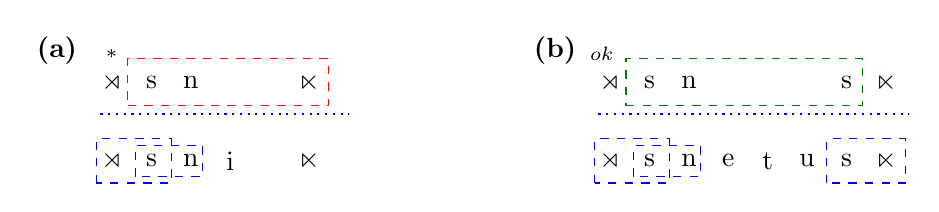
\begin{tikzpicture} %SSTSL EXAMPLE
    \node (A) at (-1.2,1.4) {\textbf{(b)}};
      \node (60) at (-0.5,0) {$\rtimes$};
        \node (0) at (0,0) {s};
        \node (1) at (0.5,0) {n};
        \node (2) at (1,0) {e};
        \node (3) at (1.5,0) {t};
        \node (4) at (2,0) {u };
        \node (5) at (2.5,0) {s};
      \node (6) at (3,0) {$\ltimes$};
        %%tier
             \node (600) at (-0.5,1) {$\rtimes$};
       \node (00) at (0,1) {s};
       \node (01) at (0.5,1) {n};
       \node (5) at (2.5,1) {s};
          \node (06) at (3,1) {$\ltimes$};
        %
        %projection function
       \draw[dashed, blue] (-0.7,-0.28 ) rectangle (0.25, 0.28);
         \draw  [dashed, blue] (-0.2,-0.2 ) rectangle (0.65, 0.2);
         \draw [dashed, blue](2.25,-0.28 ) rectangle (3.25, 0.28);
          %local constraints   
 	 \node (000) at (-0.6,1.3){$^{ok}$};
        \draw [dashed, green!50!black](-0.3, 0.7) -- (2.7, 0.7) -- (2.7,1.3) -- (-0.3,1.3) -- (-0.3, 0.7);
        %tier bar
        \draw[dotted, thick, blue] (-0.65,0.60) to (3.3,0.60);
       % \node at (-0.5,0.40) {{\tiny T}};
        
        \begin{scope}[xshift=-180pt] %string in the center
         \node (A) at (-1.2,1.4) {\textbf{(a)}};
         \node (60) at (-0.5,0) {$\rtimes$};
        \node (0) at (0,0) {s};
        \node (1) at (0.5,0) {n};
        \node (2) at (1,0) {i};
        \node (3) at (1.5,0) {\textglotstop};
         \node (6) at (2,0) {$\ltimes$};
        %%tier
          \node (600) at (-0.5,1) {$\rtimes$};
        \node (00) at (0,1) {s};
        \node (01) at (0.5,1) {n};
          \node (006) at (2,1) {$\ltimes$};
        %projection function
        \draw[dashed, blue] (-0.7,-0.28 ) rectangle (0.25, 0.28);
        \draw  [dashed, blue] (-0.2,-0.2 ) rectangle (0.65, 0.2);
	%local constraints
        \node (000) at (-0.5,1.3) {$^*$};
        \draw [dashed, red] (-0.3, 0.7) -- (2.25, 0.7) -- (2.25,1.3) -- (-0.3,1.3) -- (-0.3, 0.7);
      \draw[dotted, thick, blue] (-0.65,0.60) to (2.5,0.60);
       % \node at (-0.5,0.40) {{\tiny T}};
        %
        \end{scope}
        
        \end{tikzpicture}

%     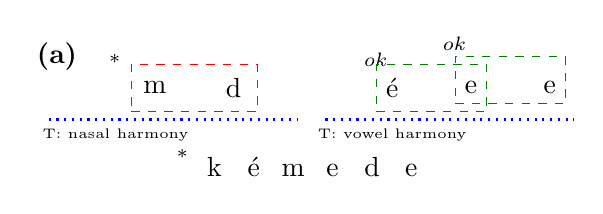
\begin{tikzpicture}

\node (A) at (-2,1.4) {\textbf{(a)}};
\node (00) at (-0.4,0.1) {$^{*}$};
\node (0) at (0,0) {k};
\node (1) at (0.5,0) {\textipa{\'e}};
\node (2) at (1,-0.05) {m};
\node (3) at (1.5,-0.05) {e};
\node (4) at (2,0) {d};
\node (5) at (2.5,-0.05) {e};
        %projection function
% \draw  [dashed, blue] (0.3,-0.28 ) rectangle (1.2, 0.28);
%\draw [dashed, blue](1.4,-0.28 ) rectangle (2.25, 0.28);
%%
\begin{scope}[xshift=50pt]
\node (1) at (0.5,1) {\textipa{\'e}};
\node (3) at (1.5,1) {e};
\node (5) at (2.5,1) {e};
%
\node (000) at (0.3,1.3) {$^{ok}$};
\draw [dashed, green!50!black] (0.3, 0.7) -- (1.7, 0.7) -- (1.7,1.3) -- (0.3,1.3) -- (0.3, 0.7);
\node (000) at (1.3,1.5) {$^{ok}$};
\draw [dashed, green!50!black] (1.3, 0.8) -- (2.7, 0.8) -- (2.7,1.4) -- (1.3,1.4) -- (1.3, 0.8);
\draw[dotted, thick, blue] (-0.35,0.60) to (2.8,0.60);
\node at (0.5,0.40) {{\tiny T: vowel harmony}};
\end{scope}
\begin{scope}[xshift=-50pt]
\node (2) at (1,1) {m};
\node (4) at (2,1) {d};
%
\node (000) at (0.5,1.3) {$^{*}$};
\draw [dashed, red] (0.7, 0.7) -- (2.3, 0.7) -- (2.3,1.3) -- (0.7,1.3) -- (0.7, 0.7);
\draw[dotted, thick, blue] (-0.35,0.60) to (2.8,0.60);
\node at (0.5,0.40) {{\tiny T: nasal harmony}};
\end{scope}
\end{tikzpicture}
  
%    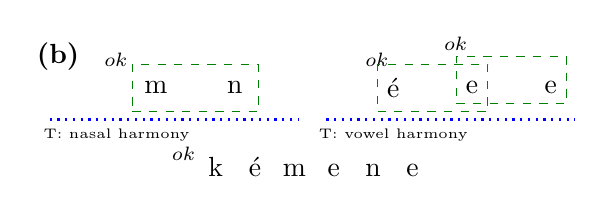
\begin{tikzpicture}

\node (A) at (-2,1.4) {\textbf{(b)}};
\node (00) at (-0.4,0.1) {$^{ok}$};
\node (0) at (0,0) {k};
\node (1) at (0.5,0) {\textipa{\'e}};
\node (2) at (1,-0.05) {m};
\node (3) at (1.5,-0.05) {e};
\node (4) at (2,-0.05) {n};
\node (5) at (2.5,-0.05) {e};
        %projection function
% \draw  [dashed, blue] (0.3,-0.28 ) rectangle (1.2, 0.28);
%\draw [dashed, blue](1.4,-0.28 ) rectangle (2.25, 0.28);
%%
\begin{scope}[xshift=50pt]
\node (1) at (0.5,1) {\textipa{\'e}};
\node (3) at (1.5,1) {e};
\node (5) at (2.5,1) {e};
%
\node (000) at (0.3,1.3) {$^{ok}$};
\draw [dashed, green!50!black] (0.3, 0.7) -- (1.7, 0.7) -- (1.7,1.3) -- (0.3,1.3) -- (0.3, 0.7);
\node (000) at (1.3,1.5) {$^{ok}$};
\draw [dashed, green!50!black] (1.3, 0.8) -- (2.7, 0.8) -- (2.7,1.4) -- (1.3,1.4) -- (1.3, 0.8);
\draw[dotted, thick, blue] (-0.35,0.60) to (2.8,0.60);
\node at (0.5,0.40) {{\tiny T: vowel harmony}};
\end{scope}
\begin{scope}[xshift=-50pt]
\node (2) at (1,1) {m};
\node (4) at (2,1) {n};
%
\node (000) at (0.5,1.3) {$^{ok}$};
\draw [dashed,  green!50!black] (0.7, 0.7) -- (2.3, 0.7) -- (2.3,1.3) -- (0.7,1.3) -- (0.7, 0.7);
\draw[dotted, thick, blue] (-0.35,0.60) to (2.8,0.60);
\node at (0.5,0.40) {{\tiny T: nasal harmony}};
\end{scope}
\end{tikzpicture}

%        \end{center}
%        % \caption{Example from Samala, allowing generalized tier projection: (a) is ill-formed because of $^*$\textipa{sn}; (b) is well-formed since  \textipa{[sn]} is followed by \textipa{[s]} later in the string. Note that \textipa{[n]} is projected on the tier only when adjacent to \textipa{[s]}.}
%         %if changed to new fig
%        \caption{Example of a MITSL analysis of  Yaka nasal and vowel harmony: (a) is ill-formed because there is a violation on the nasal harmony tier; (b) is well-formed since there are no violations on either tier.}
%        \label{fig:YAKA3}
%        \end{figure}
%
%
%%Since the ability to model multiple processes in the phonotactic of a language remains obviously desirable, it seems reasonable then to focus on the learnability of MITSL languages directly, as any algorithm able to learn an MITSL language will also trivially learn an ITSL one.
%%%%%%%%%%%%%%%%%%%
%In the rest of the paper, we directly expand of \citet{McMullinSCIL2019}'s MTSL2IA algorithm and present a grammatical inference algorithm able to learn conjunction ITSL grammars with $2$-local contexts and $2$-local tier constraints ($k$-MITSL$^2_2$), only from positive examples and without a-priori knowledge about the content or the number of tiers.
%%Since, as discussed, intersection closure if a fundamental component of natural language phonotactics, we directly expand of \citet{McMullinSCIL2019}'s MTSL2IA algorithm for MTSL$_2$ languages, and learn conjunctions of ITSL$^2_2$ languages (MITSL$^2_2$).


\section{MITSL Inference Algorithm}

The remainder of the paper discusses our learning algorithm for MITSL languages with projection contexts and tier constraints of size $2$ (MITSL$^2_2$).
While the previous section presented an intuitive definition of MITSL languages, a more formal definition is necessary in order to understand the way the algorithm works.
Thus, we first introduce some mathematical preliminaries and discuss how the definition of MITSL grammar presented in \citep{desanto2019structure}  grounds the intuition behind our generalization of \citet{McMullinSCIL2019}'s learning algorithm. 
We also discuss a generalization of the notion of  $2\text{-}path$ as introduced by \citet{JardineHeinz16}.


\subsection{Formal Preliminaries}

%symbols background
We assume familiarity with set notation on the reader's part.
Given a finite alphabet $\Sigma$, $\Sigma^*$ is the set of all possible finite strings of symbols drawn from $\Sigma$. %while $\Sigma^{\leq n}$ denotes the set of strings of length $\leq n$.
A language $L$ is a subset of $\Sigma^*$.
For every string $w$ and every non-empty string $u$, $|w|$ denotes the length of the string, $|w|_u$ denotes the number of occurrences of $u$ in $w$, and $\lambda$ is the unique empty string.
Left and right word boundaries are marked by  $\rtimes, \ltimes \notin \Sigma$ respectively.

A string $u$ is a $k$-\emph{factor} of a string $w$ iff $\exists x, y \in \Sigma^*$ such that $w=xuy$ and $|u| = k$. 
The function $\facn{k}$ maps words to the set of $k$-factors within them: $\facn{k}(w) := \{ u : u \textit{ is a $k$-factor of } w \textit{ if } |w| \geq k, \textit{ else } u = w\}$.
For example, $\facn{2}(aab) = \{ aa, ab\}$.
%
The domain of $\facn{k}$ is generalized to languages $L \subseteq \Sigma^*$ in the usual way: $\facn{k}(L) = \bigcup_{w \in L} \facn{k}(w)$.

As usual, we allow standard Boolean connectives ($\wedge$, $\vee$, $\neg$, $\rightarrow $), and first-order quantification ($\exists$, $\forall $) over individuals. 
We let $x \prec y$ denote \emph{precedence}, $x \approx y$ denote \emph{identity}, and $x, y$ denote variables ranging over positions in a finite string $w \in \Sigma^*$. Note that $\prec$ is a strict total order.
The remaining logical connectives are obtained from the given ones in the standard fashion, and brackets may be dropped where convenient. 
For example, \emph{immediate precedence} is defined as $x \triangleleft y \leftrightarrow x \prec y \wedge \neg \exists z [ x \prec z \wedge z \prec y ]$.
%
%We add a dedicated predicate for each label $\sigma \in \Sigma$ we wish to use: $\sigma(x)$ holds iff $x$ is labelled $\sigma$, where $x$ is a position in $w$.
%Classical results on definability of strings represented as finite first-order structures are then used \cite{McNaughtonPapert71}.
%If $\Sigma = \{ \sigma_1, \dots, \sigma_n \}$, then a string $w \in \Sigma^*$ can be represented as a structure $M_w$ in the signature$(\sigma_1(\cdot), \dots, \sigma_n(\cdot), \prec)$. 
%% $(P_{\sigma_1}, \dots, P_{\sigma_n}, \prec)$. 
%If $\varphi$ is a logical formula without any free variables, we use $L(\varphi) = \{ w \in \Sigma^* | M_w \text{ satisfies } \varphi \}$ as the stringset extension of $\varphi$ .

%ITSL languages
As discussed, TSL languages  have $k$-local constraints only apply to elements of a tier $T \subseteq \Sigma$.
In order to do so, a projection function (also callederasing function) is introduced to delete (or mask) all symbols that are not in $T$.
In order to extend the notion of tier in TSL languages to consider local properties of the segments in the input string, \citet{desanto2019structure} take inspiration from \cite{ChandleeHeinz18} and define ITSL projection function in terms of local contexts.
%
\begin{definition}[Contexts]
    A \emph{$k$-context} $c$ over alphabet $\Sigma$ is a triple $\tuple{\sigma, u, v}$ such that $\sigma \in \Sigma$, $u, v \in \Sigma^*$ and $|u| + |v| \leq k$.
    A \emph{$k$-context set} is a finite set of $k$-contexts.
\end{definition}
%
\begin{definition}[ISL Projection]
    Let $C$ be a $k$-context set over $\Sigma$ (where $\Sigma$ is an arbitrary alphabet also containing edge-markers).
    Then the \emph{input strictly $k$-local} (ISL-$k$) tier projection $\pi_C$ maps every $s \in \Sigma^*$ to $\pi'_C(\LeftEdge^{k-1}, s\RightEdge^{k-1})$, where $\pi'_C(u, \sigma v)$ is defined as follows, given $\sigma \in \Sigma \cup \setof{\emptystring}$ and $u,v \in \Sigma^*$:
    %
    \[
    \begin{array}{ll}
        \emptystring & \text{if } \sigma a v = \emptystring,\\
        \sigma \pi'_C(u\sigma, v) & \text{if } \tuple{\sigma, u, v} \in C,\\
        \pi'_C(u\sigma, v) & \text{otherwise.}
    \end{array}
    \]
\end{definition}
Note that an ISL-$1$ tier projection only determines projection of $\sigma$ based on $\sigma$ itself, showing that this projection function is really just an extension of what happens for TSL languages\@.
The definition of ITSL languages then  is as follows\@.

\begin{definition}[ITSL]
A language $L$ is \emph{$m$-input local $k$-TSL} ($m$-ITSL$_k$) iff there exists an $m$-context set $C$ and a finite set $R \subseteq \Sigma^k$ such that
\[
L = \{ w \in \Sigma^*: \facn{k}(\rtimes^{k-1} \pi_C(w) \ltimes^{k-1})  \cap R = \emptyset \}.
\]
A language is \emph{input-local TSL} (ITSL) iff it is $m$-ITSL$_k$ for some $k, m \geq 0$.
We call $\tuple{C, R}$ an ITSL grammar.
\label{dfn:ITSL}
\end{definition}

Note that the notion of tier is here expressed by the set of contexts C, which is the set of tier segments with the locality conditions necessary for them to be relevant to the tier constraints.
Finally, a $k$-MITSL language is defined as the intersection of $k$ ISTL languages.
The MITSL class has been shown to properly extend TSL, while remaining a proper subclass of star-free languages --- and thus subregular in its expressivity \cite{desanto2019structure}.

%Let us return to the interaction of local dissimilation and non-local harmony in Samala.
%This process can be handled by an $2$-ITSL$_3$ grammar $\tuple{S, C}$ with
%%
%\begin{itemize}
%    \item $S \is \setof{ \text{\textipa{sS}}, \text{\textipa{Ss}}, \text{\textipa{snx}} }$ where $\text{\textipa{x}} \in \{\Sigma - s\}$,
%    \item $C$ contains all of the following contexts, and only those:
%        \begin{itemize}
%            \item \tuple{\textipa{s}, \emptystring, \emptystring}
%            \item \tuple{\textipa{S}, \emptystring, \emptystring}
%            \item \tuple{\textipa{n}, \textipa{s}, \emptystring}
%        \end{itemize}
%\end{itemize}

As mentioned, in what follows we focus on learning MITSL languages with an arbitrary number of tiers, but with the locality of the contexts and of the tier-constraints fixed to $2$.
The intuition behind this paper's proposal is that, from a learning perspective, having to consider $2$-local constraints (thus a segment plus its left or right context) is equivalent to treating bigrams as unitary elements of the language, and explore dependencies over them.

%2paths
To do so, the algorithm incorporates the notion of a $2\text{-}path$ \citep{JardineHeinz16}, generalized over bigrams.
A $2\text{-}path$ is a $3$-tuple $\tup{\rho_1, X, \rho_2}$, where $\rho_1, \rho_2$  are elements in $\Sigma_{\rtimes,\ltimes}$ and $X$ is a subset of $\Sigma$.
The $2\text{-}paths$ of a strong $w = \sigma_1\sigma_2\dots\sigma_n$ are denoted $paths_2(w)$:

$$
  \begin{array}{ll}
  paths_2= \{ \tup{\sigma_i,X,\sigma_j} & |  i < j  \textit{ and}\\
   & X = \{ \sigma_z | i < z<j\} \}
    \end{array}
$$

Intuitively, a 2-path can be thought of as a precedence relation ($\rho_1\ldots{}\rho_2$) accompanied by the set $X$ of symbols that intervene between $\rho_1$ and $\rho_2$. Formally, each 2-path is therefore a 3-tuple of the form $\tup{\rho_1, X, \rho_2}$. For example, the string $\rtimes abcc\ltimes$ includes the following 2-paths: 
$\tup{a, \{\emptyset\}, b}$, $\tup{a, \{b\}, c}$, $\tup{a, \{b,c\}, c}$, $\tup{b, \{\emptyset\}, c}$, $\tup{b, \{c\}, c}$, $\tup{\rtimes, \{\emptyset\}, a}$, $\tup{\rtimes, \{a\}, b}$,  $\tup{\rtimes, \{a,b\}, c}$, $ \tup{\rtimes,\{a,b,c\},c}$, $ \tup{\rtimes,\{a,b,c\},\ltimes}$, $\tup{a, \{b,c\}, \ltimes}$, $ \tup{b, \{c\}, \ltimes}$, $\tup{c, \{c\}, \ltimes}$, $ \tup{c, \{\emptyset\}, \ltimes}$.\@
We can extend  $paths_2(\cdot)$ from strings to languages as $paths_2(L) = \bigcup_{w \in L} paths_2(w)$.

In order to have 2-paths capture the notion of context, we  have   $\rho_1, \rho_2$ be elements in $ \facn{2}(\Sigma^*_{\rtimes,\ltimes})$ and $X$ is a subset of $ \facn{2}(\Sigma)$ instead of $\Sigma$ proper.\@
The definition of $paths_2(\cdot)$ stays as above, considering $\sigma_i,\sigma_j,\sigma_z$ to be $2$-factors in $w$.\@
As this is the only notion of paths relevant for this paper, from now on we use paths, $2$-paths, or $paths_2$ interchangeably to refer this extended notion of paths over $2$-factors.
Consider once more the string $\rtimes abcc\ltimes$,  the set of  2-paths is now the following: 
$\tup{\rtimes a, \{ab\}, bc}$, $\tup{\rtimes a, \{ab,bc\}, cc}$,~$\tup{\rtimes a, \{ab,bc,cc\}, c\ltimes}$, $\tup{ab, \{bc\}, cc}$, $\tup{ab, \{bc\}, c\ltimes}$, $\tup{bc,  \{cc\}, c\ltimes}$. 

Note that  \citet{JardineHeinz16} show that the paths of a string $w$ can be calculated in time at most quadratic in the size of $w$.
This results is unaffected, once we factor the cost of generating the set of $2$-factors for $\Sigma$.


\subsection{The Algorithm}

This paper's algorithm  takes as input a set $I$ of strings over an alphabet $\Sigma$, and returns an MITSL$^2_2$ grammar $G=\bigwedge\tup{C_i,R_i}$ --- where each $C_i$ is a set of contexts in bigram formats, and each $R_i$ is a set of $2$-local constraints over contexts, represented as $4$-factors.

As mentioned before, we adopt an approach rooted in grammatical inference, following the identification in the limit learning paradigm \cite{gold1967language}, with polynomial bounds on time and data \cite{de2010grammatical}.\@
Because of this, we make the fundamental assumption that the sample data in input to the learning algorithm is a \emph{characteristic sample} for the targetted MITSL  language --- that is, it contains all the information necessary to distinguish a specific learning target (i.e., the phonological MITSL phenomenon) from any other potential targets present in the input.
In other words, we assume that the input is fully descriptive of the target pattern.

%\begin{algorithm}[!ht]
%	\KwData{A finite input sample $I\subset \Sigma^*$}
%    \KwResult{MITSL$^2_2$ grammar of the form $G=\bigwedge\tup{C_i,R_i}$}
%    Initialize $F=\facn{4}(\Sigma^*)-\facn{4}(I)$; \\
%    Initialize $B=\facn{2}(\Sigma^*)$; \\
%    	\ForEach{$f \in F$}
%        	{
%            Initialize $R_i=f$, $C_i=B$; (with $1 \leq i \leq  |F|$) \\
%             Initialize $\rho_1 = f[:2] ;\rho_2 = f[2:]$;\\
%            \ForEach{$\sigma\in B - \{f[:2], f[2:]\}$}
%            	{
%                	~\lIf {$\forall \tup{f[:2], X, f[2:]}\in paths_2(I)$ s.t. $\sigma\in X, \tup{f[:2], X-\{\sigma\}, f[2:]}\in paths_2(I)$\\}
%    					{$C_i=C_i-\{\sigma\}$ (i.e., remove $\sigma$ from $C_i$)}}
%					$G_i=\tup{C_i,R_i}$
%                }
%            $\mathbf{Return}\tn{ }G=G_1\wedge G_2\wedge ... \wedge G_{|F|}$
%            \medskip
%	\caption{Pseudocode for the MITSL$^2_2$ Inference Algorithm introduced in this paper.}
%\end{algorithm}

\begin{algorithm}[!ht]
	\KwData{A finite input sample $I\subset \Sigma^*$}
    \KwResult{MITSL$^2_2$ grammar of the form $G=\bigwedge\tup{C_i,R_i}$}
    Initialize $F=\facn{4}(\Sigma^*)-\facn{4}(I)$; \\
    Initialize $B=\facn{2}(\Sigma^*)$; \\
    	\ForEach{$f \in F$}
        	{
            Initialize $R_i=f$, $C_i=B$; (with $1 \leq i \leq  |F|$) \\
             Initialize $\rho_1 = f[:2] ;\rho_2 = f[2:]$;\\
            \ForEach{$\sigma\in B - \{\rho_1, \rho_2\}$}
            	{
                	~\lIf {$\forall \tup{\rho_1, X, \rho_2}\in paths_2(I)$ s.t. $\sigma\in X, \tup{\rho_1, X-\{\sigma\}, \rho_2}\in paths_2(I)$\\}
    					{$C_i=C_i-\{\sigma\}$ (i.e., remove $\sigma$ from $C_i$)}}
					$G_i=\tup{C_i,R_i}$
                }
            $\mathbf{Return}\tn{ }G=G_1\wedge G_2\wedge ... \wedge G_{|F|}$
            \medskip
	\caption{Pseudocode for the MITSL$^2_2$ Inference Algorithm introduced in this paper.}
\end{algorithm}

%\ForEach{$\sigma\in\Sigma - \{f[0], f[1], f[2], f[3]\}$}
Recall once again that $2$-factors (bigrams) are unitary symbols for the algorithm, and thus $2$-local tier constraints are in fact $4$-grams.
The learner exploits the fact that if a $4$-gram $\rho_1\rho_2$ is banned on some tier, then it will never appear in string-adjacent contexts.
Thus, it establishes a canonical form for an MITSL grammar by associating a tier to each individual constraint.
It then explores the specific set of contexts relevant to each specific constraint, one tier at the time, starting from the assumption that each tier projects the full set of symbols in the input string.
That is, we want to explore which symbols can act as blockers for a specific constraint.
 For each factor $\rho_1\rho_2$ absent from the training data, the goal is therefore to determine which symbols can be safely removed from the associated tier. 
 The algorithm does this by determining which bigrams are freely distributed with respect to the $4$-gram whose tier it is currently constructing.
Recall now the notion of $2$-paths, which denote precedence relations between two symbols in the language, augmented with sets of all intervening symbols.
Thus, by examining the set of $2$-paths present in the training data, we can determine which bigrams are freely distributed with respect to the $4$-gram $\rho_1\rho_2$ that is known to be banned on some tier. 
  Specifically, if all of the attested $\tup{\rho_1, X, \rho_2}$ $2$-paths that include an intervening $\sigma \in \facn{2}(\Sigma^*)$ are likewise attested \emph{without} an intervening $\sigma$, the algorithm removes that bigram from the tier, since the presence of $\rho_1\ldots{}\rho_2$ is not dependent on that intervening bigram.
Therefore , given a tier associated to the input-sensitive constraint  $\rho_1\rho_2$, only those elements that are not freely distributed with respect to  $\rho_1\rho_2$ will remain on the tier.
As the algorithm will instantiate a tier for each unattested   $\rho_1\rho_2$ in the input sample --- and  with the assumption that the input is a characteristic sample  --- this elimination procedure guarantees that the algorithms will converge to the full set of constraints and blockers for the target language.
  The crucial difference from \citet{McMullinSCIL2019}'s MTSL algorithm is that here the input sample needs to be representative of alternations between bigrams in the language, instead of elements in $\Sigma$.
  Note however that this complication is implicit within the definition of ITSL constraints, since they tie the distribution of segments in a language to their local \emph{and} non-local contexts simultaneously.
  Note that, because of this ``project everything and then remove'' strategy, the learner trivially also infers simple local constraints in the input string, which are enforced on tiers where every element of $\Sigma$ is also an element of the tier (i.e. a trivial tier).
  This is consistent with the definition of MITSL, and it is actually optimal, since it makes the algorithm truly able to capture both local and long-distance dependencies in the phonotactic of a language.

Finally, a peculiarity of our specific implementation is that the MITSL grammar returned is in its a specific canonical form.
That is, by assigning each tier to a single constraint,  it redundantly ties even  constraints that could co-exist on the same tier to distinct tiers.
Additionally, as a consequence of treating bigrams as unary symbols,  when a segment is freely distributed with respect to its contexts --- i.e., it gets projected on a tier independently on the context --- the algorithm will still treat each bigram as a distinct element.
For instance, consider $\Sigma =\{ a, e, o \}$ and assume  $e$ a tier element independently of context.
What our algorithm will infer is that any bigram containing $e$ will be a tier element, so that $C = \{ ae, ea, eo, oe, ee\}$.

In practice, it is trivially possible to add a unification step to the tier and context selection, in order to have a representation closer to the grammar a human phonologist would write.
However note that, while redundant, these two aspects of the representation learned by the algorithm are in line with our assumptions about the nature of MITSL dependencies and do not affects the ``naturalness" of the generalization.

The following section discusses the performance of the algorithm on an initial set of test data.
We also discuss how the way the algorithm instantiates tiers affects the class of learnable patterns.


\section{Evaluation\footnote{A Python implementation of the learning algorithm and testing tools is available at ADD LINK TO ANONYMOUS NOTEBOOK}}

Setting up to evaluating the algorithm, it is important to underline once again that, consistently with previous work on subregular learners,  probability plays no role in the learning approach we outlined.
As an obvious consequence, it is trivial to point out that the algorithm's generalizations are weak with respect to noisy data, since exceptions to the target pattern are treated equally to any other strings independently of their frequency.
Thus, in what follows we set up a set of preliminary evaluation cases that produce input samples devoid of exceptions.
The reader will rightfully object that this is rather unnatural for a natural language phonotactic perspective.
However, it is important to note that probabilistic approaches are not intrinsically incompatible with the MITSL learner (nor with any learner in this tradition).
For the sake of this paper though, the focus is on whether it is possible to learn MISTL$^2_2$ languages efficiently, inferring the tiers from perfect data.
This  factorization approach to the learning problem is standard in computational learning theory, as it disentangles the problem of handling noisy input from that of navigating the structure of the learning space \cite[a.o.]{OncinaGarcia91,jardine2016learning,JardineHeinz16}.

\subsection{Learnable Patterns}

We evaluate the  MISTL$^2_2$ learner on four distinct patterns representative of the classes of language the algorithm is designed to be successful over, inspecting the ability of the learner to infer grammars fully representative of the input language.
Note that we generate input samples from every language $L$ we test via random generation of strings from $\Sigma^*$ consistent with specified tier constraints.
Thus, each sample is not guaranteed to be a characteristic sample.
In this first evaluation, we set the cardinality of the input sample for each language at $1000$ --- which simulations show being sufficient for the learner to ifner the correct patter for every language analyzed.


\paragraph{An Artificial ITSL$^2_2$ Pattern} Since MITSL is a proper extension of ITSL, we first test the learner on a language with a single input-sensitive rule. Using an artificial patter instead of a (even simplified) natural language pattern allows us to keep the target generalization transparent and to use a small alphabet set. Specifically, we generate an input sample for an ITSL language $L_1$ with $\Sigma = \{a, e, o, x\}$ such that $o$ immediately before $x$ prohibits $e$ to appear anywhere in the string. 
For instance,  $eaaxaae,axaexeeexx,eaoxaao \in L_1$, while $oxaxe \notin L_1$.
The learner should infer that the correct grammar projects $o$ on the tier banning $^*oe$ iff $o$ is immediately followed by $x$, and also projects $e$ in every context.
This is exactly what the algorithm learns, with the representational peculiarities discussed above.
In particular, since the projection of $e$ is independent of context, instead of a single tier the learner instantiates a tier for every $4$-gram  $^*oxe\sigma$ and   $^*ox\sigma e$, where $\sigma$ is every element of $\Sigma = \{a, e, o, x\}$.
For each such tiers, the algorithm infers that $ox$ is always projected, as is the corresponding bigram containing $e$.
%Note that the target constraint is learned even for smaller sized of the input sample, but with a grammar that --- while perfectly compatible with the input data --- is not consistent with the original grammar originating the data.
%For instance, with an input sample of $100$ strings, the algorithm learns that $ao$ is a 

\paragraph{First-Last Harmony}
We then test a second ITSL$^2_2$ often discussed in the formal language literature on the complexity of phonotactics: an harmonic dependency between the first and the last element in the string.
For instance, assuming that the first and last symbols in a string are vowels, the requirement might be that they agree in height.
Specifically, we consider a language $L_{FL}$ with $\Sigma =\{ a, o, x\}$, and strings in$L_{FL}$  as usual enriched with start ($\rtimes$) and end ($\ltimes$) symbols.
Then, we generate data such that $^*\rtimes ao\ltimes$ $^*\rtimes oa\ltimes$ should be banned a tier.
For instance, $axaxoaxa, oaaxaxoaxo \in L_{FL}$ but  $oxaxoaxa, aaxaxoaxo \notin L_{FL}$.
This pattern is worth testing in addition to the one we used above, as it requires both elements in the constraint to be sensitive to their local context (the end and start symbol, respectively).
As expected, the learned succeeds in generalizing over the input sample, instantiating a distinct tier for each constraint combination.



\paragraph{An Artificial MTSL$^2_2$ Pattern} As the algorithm is fully successful on a single ITSL pattern, we then test it on the other relevant subclass of MITSL: as MTSL$^2_2$ language with constraints to be enforced on multiple tiers, but with a TSL projection for each tier which does not depend on context.
Specifically, we generate an artificial language $L_2$ which replicates the idea of a consonant harmony and a vowel harmony process occurring within the same language.
Specifically, we consider  $L_2$ with $\Sigma = \{a, o, p, b\}$, $T_1=\{a,o\}$, $T_2=\{p,b\}$ and enforce constraints such that $R_1 = \{^*ao, ^*oa\}, R_2= \{^*bp, ^*pb\}$.
For instance, $apapp, abbap, popooo \in L_2$ but  $apabo, appoppp \notin L_2$.
As expected, as an extension of  \citet{McMullinSCIL2019}'s MTSL inference algorithm, the learned successfully infers the full grammar.
As the algorithm still considers the patter an MITSL one, it actually needs to consider every possible context for each symbol, and it thus requires a more extensive input set than \citet{McMullinSCIL2019}'s.
For example, in order to infer ``project $a$'', the current algorithm actually learns to project \{ao, oa, ap, pa, ab, ba\}.
Importantly, this is exactly what is expected when learning an input-sensitive projection.


\paragraph{An Artificial MITSL$^2_2$ Pattern}

Once we are sure that the algorithm generalizes correctly over the appropriate subclasses, we can test it on a proper MITSL$^2_2$ pattern, which combines instances of the dependencies observed above.
In particular, we generate a language that respects two independent  ITSL$^2_2$ constraints. 
A first constraint is the one we exploited in our artificial  ITSL$^2_2$ example, such that $o$ immediately before $x$ prohibits $e$ to appear anywhere in the string.
The second constraint enforces that if $b$ immediately precedes $y$, then any following instance of $d$ is forbidden.
This replicates a simplified pattern of dissimilation.
Thus, the whole alphabet for the language is $\Sigma = \{a, e, o, x, b, p, d, y\}$ with  $ \{o, e, x\}$ being relevant only to the first constraint, and $ \{b, y, d\}$ only to the second.
This corresponds to a language $L_3$ such that $bdox,edyo,byoxpa \in L_3$ but $bydox,oxdye,byoxde \notin L_3$.
As expected given the previous results, the learner is fully successful on this language, correctly generalizing over the distinct ITSL constraints independently.
%\paragraph{Yaka Harmonies}

\subsection{Unlearnable Patterns}
\label{ssec:limits}

Our simulations show that our MTSL$^2_2$  learner succeeds on a variety complex patterns, given a positive sample representative of the target language.
However, since our approach relies directly on  \citet{McMullinSCIL2019}'s idea for instantiating multiple tiers, it suffers from the same limitations.
That is,  there is a portion of logically-possible M(I)TSL patterns which cannot be captured using the current learning strategy.
To understand why, note again that the algorithm instantiates a tier for each potential constraints.
From this, it follows immediately that  each restriction can only be enforced on at most one tier. 
Thus, the learner fails on those patters that have overlapping tier alphabets --- so tiers that share some symbols, but that are not overall in a set/subset relation.
Specifically, the algorithm is not able to consider overlapping tiers that are associated with a single \text{*}$\rho_1\rho_2$ restriction (e.g., if such constraint needs to be independently blocked by a different symbol on each tier).
It is important to note that languages exhibiting patterns with these problematic dependencies appear to be unattested, and for reasons that have been speculated to be directly related to ease of learnability, as excluding overlapping tiers exponentially reduces a learner hypothesis space \citep{aksenova2018formal}.
In this sense, algorithms of the kind presented here can help us  explicitly explore how the characteristics of subclasses of subregular languages are tied to learnability claims.

\section{Discussion}

 This paper proposes a grammatical  inference algorithm to learn multiple input-sensitive tier-based strictly local languages \citep[MITSL;][]{desanto2019structure} from positive data only, once the locality of the tier-constraints and of the tier-projection function is set to two (MITSL$^2_2$).
The algorithm makes use of the characteristics of the language class in order to guide its exploration of the learning space.
We provided a Python implementation, and discussed simulations demonstrating the learner's success over four artificial languages belonging to subclasses of MITSL$^2_2$ languages.
Thus, this paper contributes to the growing array of results for the efficient learnability of classes in the subregular hierarchy.

While the learner succeeds over languages belonging to the target class, there are several limitations towards its use as a practical learning algorithm for natural language phonotactics.
One usual critique of algorithms of this kind is the unrealistic assumptions made about the nature of the input sample.
First of all, while it is true that these algorithms are only guaranteed to converge to the correct grammar if the sample is a characteristic, that doesn't mean that the algorithm will fail in other cases.
The condition on the input comes from the fact that this learning approaches give us converging guarantees.
In this sense, our qualitative evaluation is meant as a first step toward a more extensive study of the general learning performance of these approaches, when varying the coverage of the input sample ---  in the spirit of what recently suggested in \citep{aksenova2020tool}.


Similarly, an obvious issue when applying and testing this algorithm to natural language data will come from its inability to deal with exceptions and noisy input in general.
Obviously, exceptions in the data could be handled by developing probabilistic versions of the learner. 
Note that, while formal languages were discussed here as categorical in nature, they admit stochastic counterparts.
A stochastic version of a learning algorithms for MTSL languages could for instance take into consideration the frequency of a specific path before removing a symbol from the tier.
It is also reasonable to conceive of versions of this algorithm taking natural phonotactic classes into account in order to discriminate between possible conceivable hypothesis about the a tier in presence of contradicting data.
Crucially though, the results in this paper show how inferring tiers and input-sensitive tier constraints can be achieved without \emph{a priori} information about them.
The strategy formulated here could then be combined with learning approaches that take advantage of different aspects of the nature of the input data \cite{gouskova2020inducing,rasin2019simultaneous}.

Moreover, the transparent way our algorithm explores the learning space suggests that these approaches can be used as a baseline to evaluate the needs of more opaque learning strategies with respect to different kinds of input, in line with previous work combining  grammatical inference techniques to blackbox learning models \citep[a.o.]{avcu2017subregular,mahalunkar2018using}.
Moreover, recasting ITSL structural projection as a learning problem highlighted how input-sensitive dependencies are related to symbols in the input strings, bringing intuitions that could be incorporated into other approaches to learning TSL languages and their extensions \citep{burness2020modelling}.
 
\bibliography{sstsl.bib}
\bibliographystyle{acl_natbib}



\end{document}
